%==============================================================================
%  EHRJEPA -- work-in-progress preprint
%  Build:  tectonic -X compile main.tex        (or: latexmk -pdf main.tex)
%==============================================================================
\documentclass[11pt,a4paper]{article}

\usepackage[margin=22mm]{geometry}
\usepackage[T1]{fontenc}
\usepackage[utf8]{inputenc}
\usepackage{lmodern}
\usepackage{microtype}
\usepackage{amsmath,amssymb}
\usepackage{booktabs}
\usepackage{array}
\usepackage{graphicx}
\usepackage{tikz}
\usetikzlibrary{positioning,arrows.meta,fit,backgrounds,decorations.pathreplacing,calc}
\usepackage{caption}
\usepackage{subcaption}
\usepackage{xcolor}
\usepackage[numbers,sort&compress]{natbib}
\usepackage[hidelinks]{hyperref}
\usepackage{url}
\usepackage{enumitem}
\usepackage{fancyhdr}
\usepackage[htt]{hyphenat}
\emergencystretch=3em
\hbadness=6000
\vbadness=6000

\captionsetup{font=small,labelfont=bf}
\graphicspath{{figures/}}
\setlength{\tabcolsep}{4.2pt}
\renewcommand{\arraystretch}{1.06}

\pagestyle{fancy}
\fancyhf{}
\fancyhead[L]{\footnotesize EHRJEPA --- work-in-progress preprint}
\fancyhead[R]{\footnotesize\thepage}
\renewcommand{\headrulewidth}{0.3pt}

\newcommand{\code}[1]{\texttt{\small #1}}
\newcommand{\best}[1]{\textbf{#1}}

\title{\textbf{EHRJEPA: Joint-Embedding Predictive Architectures\\
for Longitudinal Electronic Health Records}\\[4pt]
\large A work-in-progress report on five self-supervised objectives,\\
evaluated under matched compute with untrained controls}

\author{Abel Yagubyan\\
\small University of California, Berkeley\\
\small \texttt{abelyagubyan@berkeley.edu}}

\date{6 September 2026}

%==============================================================================
\begin{document}
\maketitle
\thispagestyle{fancy}

\begin{center}
\fbox{\parbox{0.93\textwidth}{\small
\textbf{Status: work in progress.} This document reports the state of an ongoing
project. Every number in it comes from a run recorded in the project
repository at a named commit. All pretraining is on a single synthetic,
claims-derived source (CMS DE-SynPUF) with no laboratory values; no
experiment on MIMIC-IV or EHRSHOT has been run. The largest token budget
reported (1B) now has three training seeds per cell for \code{ar} and the
hybrid, re-scored on the full 11{,}708-subject held-out split; the 200M
budget, and \code{recon\_only} and \code{jepa\_ema} at every budget they were
run at, remain one training seed on the earlier 3{,}000-subject held-out
subset. Nothing here
should be read as a statement about what these objectives do at production
scale or on clinical data.}}
\end{center}

\vspace{2mm}

%==============================================================================
\begin{abstract}
\noindent
We implement and compare five self-supervised objectives over longitudinal
electronic health record (EHR) event streams in MEDS format: masked-span
latent joint-embedding prediction (JEPA), causal next-latent JEPA,
window-pooled latent JEPA, next-code autoregression (AR), and a hybrid that
carries a dense next-latent term and the next-code term through one trunk. All
variants share an event embedding that fuses a learned code embedding with a
value quantizer and Fourier time features, a rotary-position encoder, and, for
the latent objectives, a stop-gradient target encoder regularized against
collapse by a SIGReg-style distributional penalty. We evaluate frozen-encoder
probes on seven downstream tasks defined declaratively through ACES, against
count-feature logistic-regression and gradient-boosting baselines and against
architecture- and pooling-matched untrained (\code{random\_init}) controls, on
a fixed seeded 3{,}000-subject held-out cut with 200 bootstrap resamples.

Across 20 pilot cells trained to a matched 48M-token budget, the five
masked-span JEPA variants score mean AUROC 0.6776--0.6901 against a shared
untrained control at 0.6821 (gain $-0.0046$ to $+0.0080$), while next-code AR
scores 0.7205 against its own control at 0.6760 ($+0.0445$). Adding an
auxiliary code-reconstruction term to a masked-span JEPA raises the gain to
$+0.0177$ to $+0.0296$; removing the latent term entirely and keeping only
code reconstruction retains $+0.0254$. The dense causal hybrid scores 0.7287
($+0.0923$), the highest of the 20 cells. Scaling the hybrid and AR to 200M
and 1B nominal token slots on a 6-layer, 256-wide encoder, on a fixed
3{,}000-subject held-out subset, the hybrid improves at every step (0.7287,
0.7328, 0.7363, the last a 3-seed mean) while AR does not improve from 200M
to 1B (0.7304, 0.7251, the last a 3-seed mean). A fourth ablation grid finds
that two independently measured +0.6-point gains (dropping SIGReg; a frozen
AR teacher in place of EMA) do not stack when combined (mean-of-six-task
AUROC 0.7625 combined against 0.7615 for either alone), which fixes the
repository default's target encoder as EMA. \textbf{Re-scored on the FULL
11{,}708-subject held-out split, at 1B tokens and three seeds, this default
--- hybrid, causal, horizons $[1,4,16]$, no SIGReg, EMA target --- scores
mean AUROC 0.763 across six non-mortality tasks against AR's 0.744, with
per-task seed ranges non-overlapping on all six, and above \code{gbm} (0.751)
and \code{lr} (0.719) on the same split; this full-split comparison
supersedes the 3{,}000-subject-subset numbers above for every cell it
covers.} Three pre-registered diagnostics
measured on the
masked-span checkpoints are reported: a ridge map from mask-token time
features alone recovers $R^2 = 0.58$ of the layer-normed targets against 0.79
for the trained predictor with context; a linear code-identity probe reads
top-1 0.50 off the trained JEPA encoders against 0.60 off an untrained
encoder and 0.71 off the AR encoder; and without SIGReg a plain context-mean
baseline reaches cosine 0.73 to the targets. We report what the evidence
supports and what it does not. Every pure latent-prediction variant tested
loses to next-code prediction at matched compute; the hybrid's dense latent
term is worth about two points of mean AUROC over AR alone at 1B tokens on
the full split, three points on \code{readmission\_30d}, and about three
points at $k{=}32$ few-shot, but the gain is not observed with the code loss
removed. Whether a latent objective does work of its own on continuous,
high-entropy targets, rather than riding on a code-prediction loss over
discrete, low-entropy events, is untested here; a pre-registered comparison on
two continuous hourly-ICU-state datasets, with a decision rule fixed before
training, is specified in Section~\ref{sec:a2} and
\code{docs/experiments/A2\_PLAN.md} and has not yet been run.
\end{abstract}

\vspace{2mm}

%==============================================================================
\section{Introduction}

An electronic health record is a stream of timestamped clinical events ---
diagnoses, procedures, medication fills, admissions, laboratory results ---
observed at irregular intervals over years. The dominant self-supervised recipe
for such data is next-token autoregression over a serialized code sequence, in
the manner of CLMBR \citep{ehrshot}, ETHOS \citep{ethos}, CEHR-GPT
\citep{cehrgpt} and EHRMamba \citep{ehrmamba}. That recipe inherits a property
of language modelling that is less obviously appropriate here: it spends its
entire capacity on predicting the identity of the next discrete symbol,
including the large fraction of symbol identity that is administrative,
arbitrary, or genuinely unpredictable. Which of several thousand billable codes
a clinician selects for the same underlying condition, and which of many
interchangeable national drug codes a pharmacy dispenses, are not facts a
representation of the patient needs to carry.

\paragraph{What JEPA promises for EHR.}
Joint-embedding predictive architectures \citep{ijepa,vjepa2} sidestep this by
predicting in representation space. A context encoder reads the observed
events; a predictor, conditioned on where and when the unobserved events fall,
predicts the \emph{representations} a target encoder assigns to them; nothing is
reconstructed in input space. The target is produced by a stop-gradient copy of
the encoder, so the objective is free to discard detail that is not predictable
--- exactly the detail an EHR stream is full of. The obvious failure mode,
representational collapse, is addressed here by SIGReg \citep{lejepa}, which
pushes embeddings toward an isotropic Gaussian through random one-dimensional
projections rather than through architectural asymmetry or negative pairs. On
paper this is a good match for clinical event streams. This paper reports what
happened when we measured it.

\paragraph{Contributions.}
Stated as facts about what exists and what was measured, not as claims about
importance:

\begin{enumerate}[leftmargin=*,itemsep=2pt,topsep=3pt]
\item An open implementation of five objective families over a common MEDS
      \citep{meds} data path, a common event embedding, and a common encoder:
      masked-span latent JEPA, causal next-latent JEPA, window-pooled latent
      JEPA, next-code AR, and an AR/JEPA hybrid (Section~\ref{sec:model}).
\item A downstream evaluation harness in which every model sees identical
      anchors and identical history windows, history is cut by a single strict
      inequality, tasks are defined declaratively in ACES \citep{aces}, and
      every trained cell is scored against an architecture- and pooling-matched
      untrained control as well as against count-feature baselines
      (Section~\ref{sec:eval}).
\item Five ablation grids at a matched 48M-token budget --- 20 trained cells at
      seed 0, plus four seed-replication cells --- and two token-scaling grids
      at 200M and 1B nominal token slots, the 1B grid replicated at three
      seeds each for \code{ar} and the hybrid (Section~\ref{sec:experiments}).
\item The measured result that, at these budgets on this source, masked-span
      latent prediction alone does not move a frozen-encoder probe past its own
      untrained control, that an auxiliary discrete code term recovers most of
      the gain the latent term does not produce, and that a dense causal
      next-latent term stacked on next-code AR scores above either component
      alone at all three budgets.
\item Three diagnostics measured before the grids that were designed against
      them, each identifying a route by which the masked-span objective can be
      satisfied without the encoder carrying information a probe would want
      (Section~\ref{sec:diagnostics}).
\end{enumerate}

\paragraph{What this paper is not.}
It is not a benchmark result. DE-SynPUF is a synthetic public-use file
constructed by sampling and swapping fields across real Medicare beneficiaries
specifically in order to break re-identifiable associations, so the predictive
structure between a patient's history and their future is weakened by
construction. The absolute AUROCs below are a property of that source and are
not comparable to published numbers on MIMIC-IV or EHRSHOT. What the design
supports are \emph{relative} comparisons at matched compute, on identical rows,
with an untrained control and a count-feature ceiling computed on the same
rows.

%==============================================================================
\section{Related work}
\label{sec:related}

\paragraph{Foundation models for structured EHR.}
CLMBR-style autoregressive pretraining over serialized clinical codes, together
with the EHRSHOT few-shot benchmark, established the evaluation shape this work
follows \citep{ehrshot}. MOTOR \citep{motor} pretrains on time-to-event
targets rather than next-code identity. ETHOS \citep{ethos} and CEHR-GPT
\citep{cehrgpt} pursue generative patient-timeline modelling, the latter with
explicit temporal tokens; EHRMamba \citep{ehrmamba} substitutes a state-space
backbone for attention. Delphi-2M \citep{delphi2m} models disease progression
generatively at population scale. \citet{contextclues} study what long-context
architectures over EHR event streams actually use their context for, which is
the question our diagnostics in Section~\ref{sec:diagnostics} ask of a latent
objective. \citet{ehrscaling} report scaling behaviour for EHR foundation
models, and \citet{tokenization} study how tokenization choices trade off
against downstream quality --- both directly relevant to the vocabulary
construction in Section~\ref{sec:data} and the token-budget grids in
Section~\ref{sec:scale}.

\paragraph{Data and task standards.}
MEDS \citep{meds} is the interchange format every source in this project is
lowered into; ACES \citep{aces} evaluates the cohort and label windows from
declarative YAML, so the seven tasks below are specified rather than
implemented. MEDS-Tab \citep{medstab} is the tabularization baseline our
count-feature construction deliberately mirrors.

\paragraph{Joint-embedding prediction.}
I-JEPA \citep{ijepa} introduced masked latent prediction with a stop-gradient
target encoder; V-JEPA~2 \citep{vjepa2} extends it to video at scale. LeJEPA
\citep{lejepa} replaces heuristic anti-collapse machinery with SIGReg, an
explicit isotropic-Gaussian penalty estimated through random one-dimensional
projections, and is the formulation this implementation follows;
\citet{salt} report that the teacher branch can be frozen without loss, which
our \code{shared}-versus-\code{ema} ablation asks in a different form and
Section~\ref{sec:ablate3}'s frozen-AR-teacher cell tests directly. LeNEPA
\citep{lenepa} pursues next-latent prediction for time
series without augmentation, which is structurally the objective family
(b) below arrives at from a different direction.

\paragraph{JEPA and world models for clinical data.}
\citet{tsjepa} apply joint-embedding prediction to general time series.
Clin-JEPA \citep{clinjepa} pretrains a joint-embedding predictive objective on
EHR patient trajectories directly, and \citet{smbstructure} argue for a
world-model rather than document-modelling framing of the longitudinal record;
FoMoH \citep{fomoh} proposes a clinically-grounded evaluation for structured-EHR
foundation models. The masked-span variant in Section~\ref{sec:objectives} is
the closest analogue to that line, and is the variant that does not clear its
untrained control at the budgets reported here.

%==============================================================================
\section{Data and representation}
\label{sec:data}

\subsection{Canonical MEDS layout}

Three sources are supported and each is lowered once into one identical on-disk
shape, so that no component downstream of the ETL learns that more than one
source exists: MIMIC-IV (credentialed, via PhysioNet), CMS DE-SynPUF (public
use), and Synthea (generated). Shards carry the MEDS~0.4 core columns
--- \code{subject\_id}, \code{time}, \code{code}, \code{numeric\_value},
\code{text\_value} --- sorted by \code{(subject\_id, time, code)} with null
times first, so a subject's static facts precede their timeline. Shards are
subject-disjoint. Source-specific extension columns are dropped rather than
carried; \code{meds\_etl}'s MIMIC output has roughly twenty of them, and keeping
them would mean the model sees a different column set per source. Every shard
is validated against the MEDS schema before it is written.

Splits are a pure function of the subject identifier:
\code{blake2b("split:\textless seed\textgreater:\textless subject\_id\textgreater")}
truncated to 64 bits, taken modulo 10{,}000 and cut at 8000/9000 for an
80/10/10 train/tuning/held-out draw, with the seed pinned at 20240917 by a
test. Codes are \emph{not} harmonised across sources --- there is no shared
ontology mapping step, and inventing one would be guesswork --- but the shape
\code{NAMESPACE//value} is.

\paragraph{The source used for every experiment below.}
All results in this paper are on \code{desynpuf-s1}: 116{,}352 subjects and
14.2M events in MEDS form. DE-SynPUF is a claims-derived file. It contains
diagnoses (ICD-9-CM), procedures (ICD-9 procedure, HCPCS), drug events (NDC),
admissions, discharges with length of stay, DRGs, and beneficiary
demographics. \textbf{It contains no laboratory results, no vital signs, and no
clinical notes.} The set of event types available to the model is therefore
narrower than in a typical clinical extract, and the value channel is sparsely
populated (length of stay in days, days supplied).

\subsection{Tokenization}

One MEDS event becomes one token. The vocabulary and the value quantizer are
fit on the \code{train} split only and then reused for \code{tuning} and
\code{held\_out}. Three steps produce the vocabulary:

\begin{enumerate}[leftmargin=*,itemsep=2pt,topsep=3pt]
\item \textbf{Normalization.} \code{NDC//\textless digits\textgreater} is
      truncated to its first nine characters. An 11-digit NDC is
      labeler(5)+product(4)+package(2); the package segment records whether the
      bottle held 30 tablets or 90. Numerically this dominates everything else:
      266{,}653 of DE-SynPUF's 288{,}274 distinct training codes are NDCs, and
      folding to nine digits leaves 138{,}443 distinct codes.
\item \textbf{Hierarchical rollup before \code{[UNK]}.} Ids 0--3 are
      \code{[PAD]}, \code{[UNK]}, \code{[CLS]}, \code{[MASK]}. A code with at
      least 5 training occurrences gets its own id. A rarer code is truncated
      towards an ancestor that is frequent enough: ICD codes strip one
      character at a time (\code{ICD9CM/250.01} $\to$ \code{250.0} $\to$
      \code{250} $\to$ \code{25} $\to$ \code{2}), NDC falls back to the 5-digit
      labeler, HCPCS to its first three characters, anything else to the bare
      prefix, and only then to \code{[UNK]}. Admission is one bottom-up sweep
      in which a node holds its own count plus the mass of its \emph{rejected}
      children, so mass is never counted at two levels at once.
\item \textbf{The cap.} \code{--max-vocab 30000} bounds the table; entries are
      demoted smallest-mass-first, each demotion handing its whole mass to the
      nearest still-admitted ancestor.
\end{enumerate}

On DE-SynPUF at 30{,}000 rows (from 252{,}935 uncapped), the \code{[UNK]} rate
is 0.0 on every split --- every DE-SynPUF code has a prefix in the table to fall
back to --- and the fallback-to-ancestor rate is 16.2\% train, 16.3\% tuning,
16.5\% held-out.

\paragraph{Value quantizer.}
A raw float is meaningless without its code, so quantization is per code. Every
vocabulary id with at least 20 training observations gets nine interior decile
edges plus a mean and standard deviation; ids below that share their prefix's
fit, and failing that a global one. Non-negative codes with $|\text{skew}| > 2$
are $\log(1+x)$-transformed before the moments are taken. A value sitting
exactly on an edge falls in the \emph{lower} bin, which keeps a code whose
values are mostly one constant from smearing across bins.

\paragraph{Per-event features.}
Table~\ref{tab:features} lists what the cache stores per event. Subjects with no
\code{MEDS\_BIRTH} are anchored at their first event and flagged, so a model can
learn not to trust their ages. Events with identical timestamps get
$\log\Delta = 0$ and keep their source order.

\begin{table}[t]
\centering\small
\caption{Per-event features in the tensor cache. One MEDS event becomes one
token. \code{time\_min} is not a model input; it is what the evaluation harness
binary-searches to cut history at an anchor.}
\label{tab:features}
\begin{tabular}{llp{0.60\textwidth}}
\toprule
feature & dtype & meaning \\
\midrule
\code{code\_id}   & int32   & vocabulary id, after hierarchical fallback \\
\code{value\_bin} & int8    & 0 = no numeric value; 1--10 = decile of the code's training values \\
\code{value\_z}   & float32 & $z$-score of the (optionally $\log 1p$-ed) value, clipped to $\pm 5$; 0 when absent \\
\code{age}        & float32 & years since \code{MEDS\_BIRTH}, clipped to $[0, 120]$ \\
\code{log\_delta} & float32 & $\log 1p$ of hours since the subject's previous event; 0 for the first event and for ties \\
\code{time\_min}  & int64   & raw event time, minutes since epoch, for label alignment only \\
\bottomrule
\end{tabular}
\end{table}

Feature arrays are written as one flat memory-mapped vector per split with a
side table giving each subject's offset and length, so a training run pages in
only the windows it samples. \code{EventSequenceDataset} yields one item per
subject; \code{sampling="random\_window"} draws a fresh contiguous window on
each request. On this cache the \code{train} split holds 78{,}997 subjects
after dropping those with fewer than 16 events (13{,}995 dropped) and 11.3M
events; a \code{max\_len} 256 window averages 121 real events (47\% fill,
measured over 2{,}000 draws).

%==============================================================================
\section{Model and objectives}
\label{sec:model}

\begin{figure}[t]
\centering
\resizebox{\textwidth}{!}{% Architecture: event embedding -> context encoder -> predictor, with the
% stop-gradient target branch and the three loss terms.
% Requires: tikz + arrows.meta.  Wrap in \resizebox to fit \textwidth.
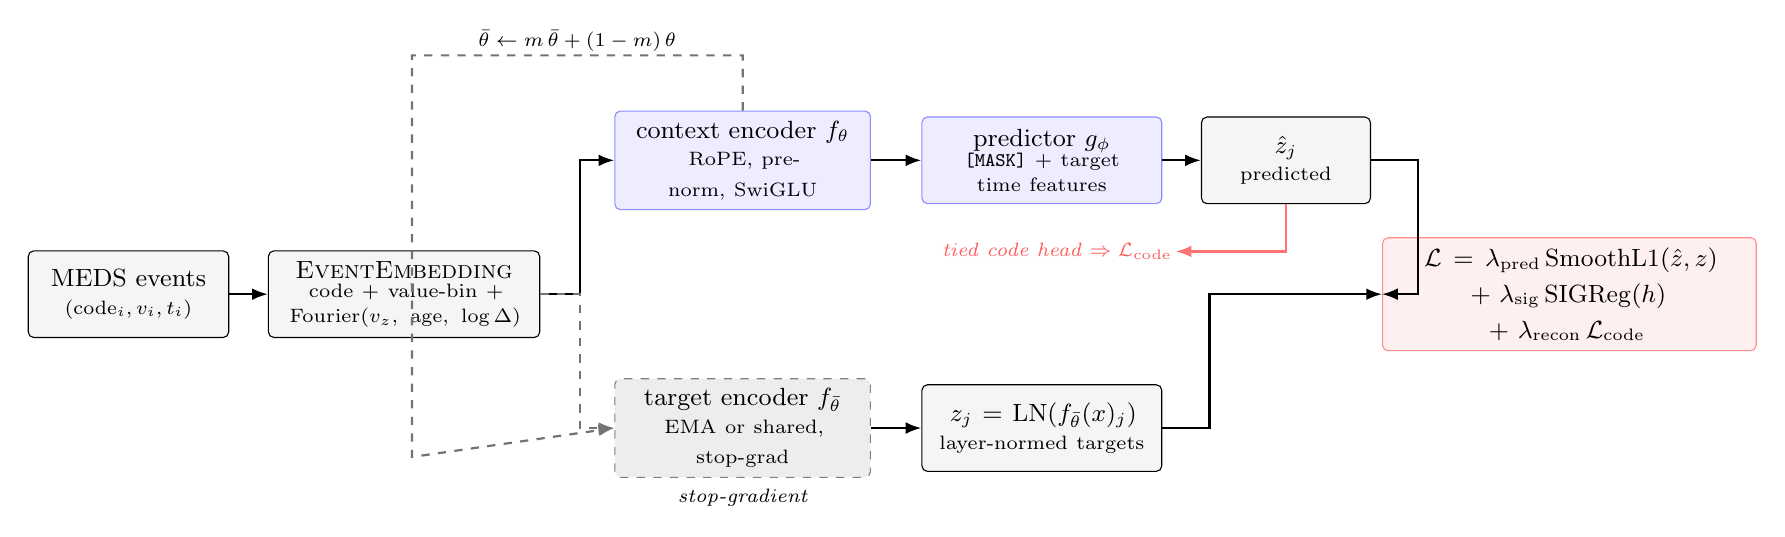
\begin{tikzpicture}[
  font=\small,
  box/.style   = {draw, rounded corners=2pt, align=center, inner sep=3.5pt,
                  minimum height=11mm, fill=white},
  data/.style  = {box, fill=black!4},
  net/.style   = {box, fill=blue!7, draw=blue!45},
  frz/.style   = {box, fill=black!7, draw=black!50, dashed},
  loss/.style  = {box, fill=red!6, draw=red!45},
  fl/.style    = {-{Latex[length=2mm]}, thick},
  sg/.style    = {-{Latex[length=2mm]}, thick, dashed, draw=black!55},
  lbl/.style   = {font=\scriptsize\itshape, inner sep=1pt},
]

% ---------------- shared trunk -----------------------------------------
\node[data, text width=23mm] (ev)  at (0mm,   0mm)
  {MEDS events\\[-1pt]{\scriptsize $(\mathrm{code}_i, v_i, t_i)$}};

\node[data, text width=32mm] (emb) at (35mm,  0mm)
  {\textsc{EventEmbedding}\\[-1pt]{\scriptsize code $+$ value-bin $+$\\[-2pt]
   Fourier$(v_z,\ \mathrm{age},\ \log\Delta)$}};

% ---------------- online branch (top) ----------------------------------
\node[net, text width=30mm]  (ctx) at (78mm,  17mm)
  {context encoder $f_\theta$\\[-1pt]{\scriptsize RoPE, pre-norm, SwiGLU}};

\node[net, text width=28mm]  (prd) at (116mm, 17mm)
  {predictor $g_\phi$\\[-1pt]{\scriptsize \texttt{[MASK]} $+$ target\\[-2pt]
   time features}};

\node[data, text width=19mm] (ph)  at (147mm, 17mm)
  {$\hat z_j$\\[-1pt]{\scriptsize predicted}};

% ---------------- target branch (bottom) -------------------------------
\node[frz, text width=30mm]  (tgt) at (78mm, -17mm)
  {target encoder $f_{\bar\theta}$\\[-1pt]{\scriptsize EMA or shared, stop-grad}};

\node[data, text width=28mm] (tz)  at (116mm,-17mm)
  {$z_j = \mathrm{LN}\!\left(f_{\bar\theta}(x)_j\right)$\\[-1pt]
   {\scriptsize layer-normed targets}};

% ---------------- loss --------------------------------------------------
\node[loss, text width=45mm] (ls) at (183mm, 0mm)
  {$\mathcal{L} = \lambda_{\mathrm{pred}}\,\mathrm{SmoothL1}(\hat z, z)$\\[2pt]
   $+\ \lambda_{\mathrm{sig}}\,\mathrm{SIGReg}(h) $\\[2pt]
   $+\ \lambda_{\mathrm{recon}}\,\mathcal{L}_{\mathrm{code}}$};

% ---------------- edges -------------------------------------------------
\draw[fl] (ev) -- (emb);
\draw[fl] (emb.east) -- ++(5mm,0) |- (ctx.west);
\draw[sg] (emb.east) -- ++(5mm,0) |- (tgt.west);
\draw[fl] (ctx) -- (prd);
\draw[fl] (prd) -- (ph);
\draw[fl] (tgt) -- (tz);
\draw[fl] (ph.east) -- ++(6mm,0) |- (ls.west);
\draw[fl] (tz.east) -- ++(6mm,0) |- (ls.west);

% EMA feedback: online weights -> target weights, around the right side
\draw[sg] (ctx.north) -- ++(0,7mm) -- ++(-42mm,0)
          node[lbl, above, midway] {$\bar\theta \leftarrow m\,\bar\theta + (1-m)\,\theta$}
          -- ++(0,-51mm) -- (tgt.west);

% code-reconstruction tap
\draw[fl, draw=red!55] (ph.south) -- ++(0,-6mm) -- ++(-14mm,0)
  node[lbl, left, align=right, text=red!65]
  {tied code head $\Rightarrow \mathcal{L}_{\mathrm{code}}$};

\node[lbl, below=1mm of tgt] {stop-gradient};

\end{tikzpicture}
}
\caption{The shared architecture. The context encoder $f_\theta$ and the
predictor $g_\phi$ carry gradients; the target encoder $f_{\bar\theta}$ runs
under stop-gradient, either as a weight-shared copy or as an EMA copy, and is
never told what code or value the masked span holds. Nothing is reconstructed
in input space by the latent term; the optional code-reconstruction term
$\mathcal{L}_{\mathrm{code}}$ passes the \emph{predicted} latent through the
tied code head.}
\label{fig:arch}
\end{figure}

\subsection{Event embedding}

For event $i$ with code id $c_i$, value bin $b_i$, standardized value $z_i$,
age $a_i$ and log inter-event gap $d_i$, the input token is a \emph{sum} ---
nothing is concatenated:
\begin{equation}
x_i \;=\; E_{\mathrm{code}}[c_i] \;+\; E_{\mathrm{bin}}[b_i]
      \;+\; \mathbb{1}[b_i \neq 0]\cdot g_{v}(z_i)
      \;+\; m_i\big(g_{a}(a_i) + g_{\delta}(d_i)\big),
\label{eq:embed}
\end{equation}
followed by dropout. The gate $\mathbb{1}[b_i \neq 0]$ exists because
\code{value\_z} is stored as $0.0$ for value-less events and $0.0$ is also an
ordinary $z$-score; without it, ``no value'' and ``exactly average'' would
collide. The factor $m_i \sim \mathrm{Bernoulli}(1 - p_{\mathrm{tdrop}})$ is
per-token time-feature dropout, applied during training only and only in the
cells that use it.

Each $g_\bullet$ is an independent two-layer network over a fixed Fourier
featurization of its scalar,
\begin{equation}
\begin{aligned}
g(u) &\;=\; W_2\,\mathrm{GELU}\!\left(W_1\,\phi(u) + b_1\right) + b_2, \\[2pt]
\phi(u) &\;=\; \big[\sin(2\pi f_1 u), \ldots, \sin(2\pi f_K u),\;
               \cos(2\pi f_1 u), \ldots, \cos(2\pi f_K u)\big],
\end{aligned}
\end{equation}
with $K = 16$ frequencies log-spaced from $10^{-2}$ to $10^{1}$ cycles per input
unit, so periods span 100 down to 0.1 units, and a hidden width equal to the
model width. Note the layout: all sines then all cosines, not interleaved. Time
therefore enters the model \emph{twice and differently} --- as a \emph{content}
feature through $g_a$ and $g_\delta$, and as \emph{position} through rotary
embeddings inside attention. That separation is what makes the \code{notime}
ablations of Section~\ref{sec:experiments} possible: the content path can be
switched off while the positional path remains.

\subsection{Encoder, predictor, target encoder}

\paragraph{Encoder.}
A pre-norm transformer: $x \leftarrow x + \mathrm{Attn}(\mathrm{LN}(x))$ then
$x \leftarrow x + \mathrm{MLP}(\mathrm{LN}(x))$, with a final LayerNorm after
the last block. Attention uses one fused QKV projection and rotary position
embeddings (base $10^4$) applied to queries and keys only; positions are
\emph{sequence indices}, not wall-clock, since irregular spacing is already
carried by $g_\delta$. The feed-forward is SwiGLU,
$\mathrm{MLP}(x) = W_3\big((W_1 x)\odot\mathrm{SiLU}(W_2 x)\big)$, at hidden
width $8\cdot\mathrm{round}(\tfrac{2}{3}\cdot\tfrac{d\,r}{8})$ for ratio
$r = 4$. Dropout is 0.1; attention dropout is 0. A learned \code{[CLS]} token is
prepended at index 0. Padding is masked key-side only. The encoder runs
bidirectionally for the masked-span objectives and causally (a lower-triangular
mask intersected with the padding mask) for AR, next-latent and window. One
consequence matters downstream: under a causal mask the \code{[CLS]} output row
is a function of the \code{[CLS]} parameter alone --- a prefix token cannot read
the sequence without leaking the future back at the next layer --- which is why
the evaluation probe uses the last valid token rather than \code{[CLS]} for
causal checkpoints.

\paragraph{Predictor (masked-span only).}
A narrower transformer over one sequence of the encoder's original length, with
no \code{[CLS]}. Each position is one of three things: a \emph{context}
position, carrying the encoder output projected to the predictor width; a
\emph{target} position, carrying a mask token; or \emph{dropped}, excluded from
attention and zeroed. A mask token is
\begin{equation}
t_i \;=\; \texttt{[MASK]} \;+\; P\big(g^{\mathrm{pred}}_{a}(a_i)
                                      + g^{\mathrm{pred}}_{\delta}(d_i)\big),
\end{equation}
carrying the \emph{target's} time and nothing else about it; with
\code{mask\_token\_time: false} the second term is dropped and every target's
token is the same vector, distinguished only by rotary position at its original
index. Attention inside the predictor is bidirectional over
context $\cup$ target, and the output is projected back to encoder width. No
target content reaches the predictor by any route: not through the mask tokens,
and not through the context representations, because the context encoder pass
never attended to target positions. A unit test asserts this numerically by
perturbing target codes and values and checking the predictions are
bit-identical.

\paragraph{Target encoder.}
A stop-gradient copy of the embedding and encoder in one of two modes.
\code{shared} evaluates the online weights under \code{no\_grad}: there is no
second copy and nothing to schedule, and collapse is prevented by SIGReg alone.
\code{ema} --- used by every configuration reported here --- keeps a frozen
deep copy whose parameters track the online ones,
\begin{equation}
\bar\theta \;\leftarrow\; m(t)\,\bar\theta \;+\; \big(1 - m(t)\big)\,\theta,
\qquad
m(t) \;=\; m_0 + (m_1 - m_0)\,\mathrm{clip}\!\left(\tfrac{t}{T}, 0, 1\right),
\end{equation}
with buffers copied rather than averaged. The momentum schedule is
\emph{linear}, not cosine, from $m_0 = 0.996$ to $m_1 = 1.0$ over the run's step
count, so the target network freezes exactly at the end of the run. Stop-gradient
is enforced three ways: \code{requires\_grad\_(False)} on the copy,
\code{no\_grad} on the target pass, and \code{.detach()} on the returned tensor.
Time-feature dropout is set to zero on the target side --- it is an augmentation
of the online input only.

\subsection{The objectives}
\label{sec:objectives}

\begin{figure}[t]
\centering
\resizebox{0.98\textwidth}{!}{% The five objective families, drawn on a common 12-token strip.
% Blue = observed context, red = predicted / supervised, grey dashed = masked.
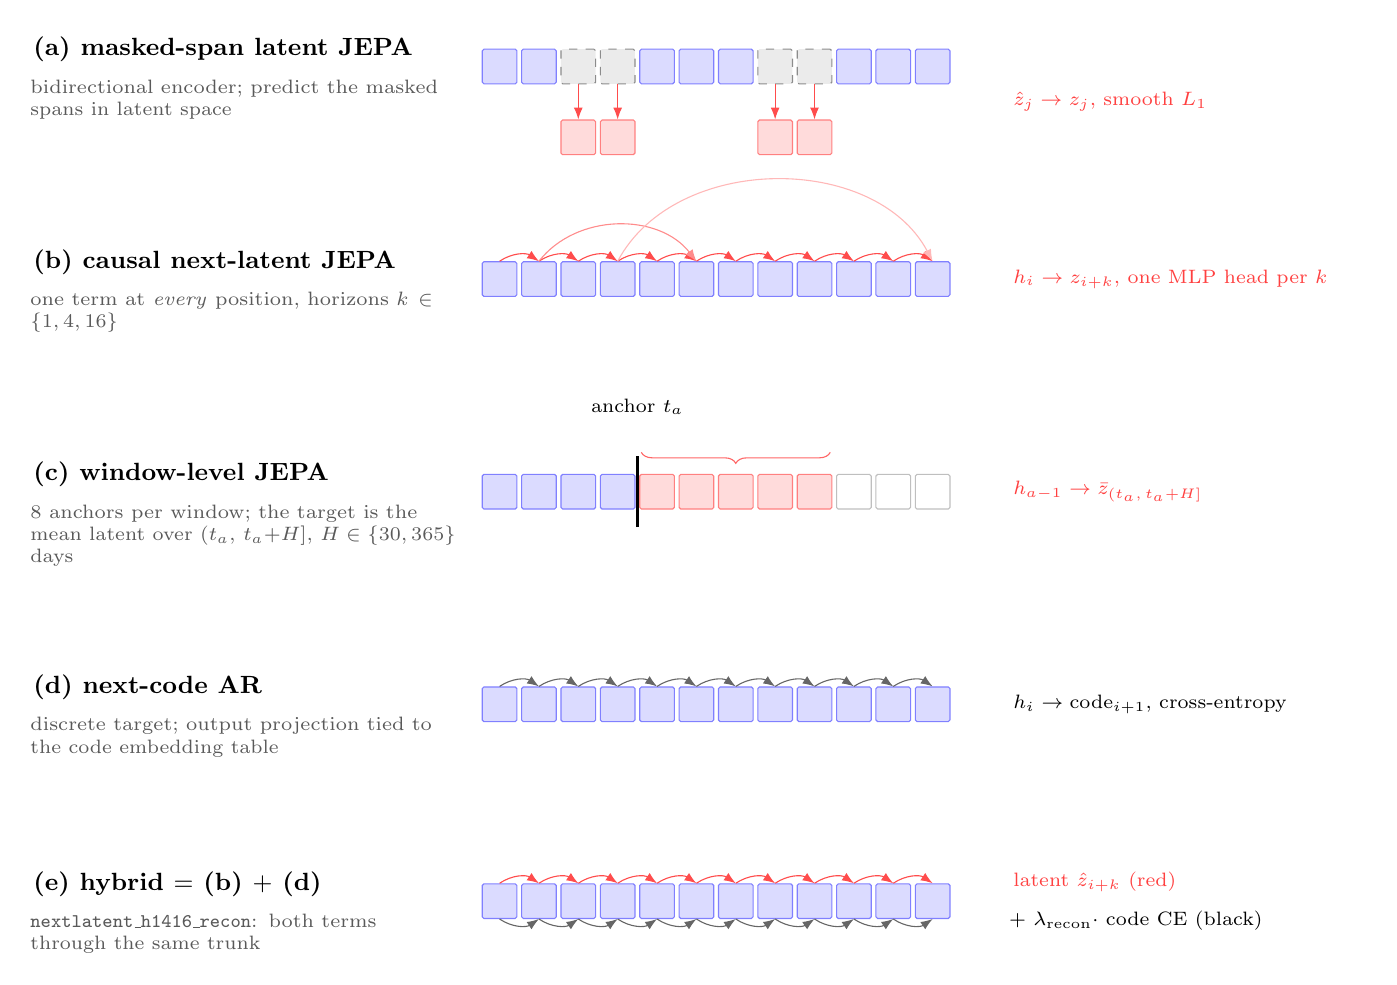
\begin{tikzpicture}[
  font=\small,
  tok/.style  = {draw, minimum width=4.4mm, minimum height=4.4mm, inner sep=0pt,
                 rounded corners=0.6pt},
  ctx/.style  = {tok, fill=blue!14, draw=blue!50},
  tgt/.style  = {tok, fill=red!14,  draw=red!50},
  msk/.style  = {tok, fill=black!8, draw=black!45, dashed},
  nul/.style  = {tok, fill=white,   draw=black!25},
  ttl/.style  = {font=\small\bfseries, anchor=north west, text width=54mm},
  sub/.style  = {font=\scriptsize, anchor=north west, text width=54mm,
                 text=black!65, inner sep=1pt},
  rhs/.style  = {font=\scriptsize, anchor=west, text width=44mm},
  ar/.style   = {-{Latex[length=1.5mm]}, thin, draw=red!70},
  arb/.style  = {-{Latex[length=1.5mm]}, thin, draw=black!60},
]

\newcommand{\strip}[2]{%  #1 = node prefix, #2 = comma list of styles
  \foreach \s [count=\i from 0] in {#2} {
    \node[\s] (#1\i) at (\i*5mm, 0) {};
  }%
}

% ======================= (a) masked-span latent JEPA ===================
\begin{scope}
  \node[ttl] (ta) at (-60mm,  5mm) {(a) masked-span latent JEPA};
  \node[sub, below=0.6mm of ta.south west, anchor=north west]
    {bidirectional encoder; predict the masked spans in latent space};
  \strip{a}{ctx,ctx,msk,msk,ctx,ctx,ctx,msk,msk,ctx,ctx,ctx}
  \foreach \i in {2,3,7,8} {
    \node[tgt] (at\i) at (\i*5mm,-9mm) {};
    \draw[ar] (a\i.south) -- (at\i.north);
  }
  \node[rhs, text=red!75] at (64mm, -4.5mm) {$\hat z_j \to z_j$, smooth $L_1$};
\end{scope}

% ======================= (b) causal next-latent ========================
\begin{scope}[yshift=-27mm]
  \node[ttl] (tb) at (-60mm,  5mm) {(b) causal next-latent JEPA};
  \node[sub, below=0.6mm of tb.south west, anchor=north west]
    {one term at \emph{every} position, horizons $k \in \{1,4,16\}$};
  \strip{b}{ctx,ctx,ctx,ctx,ctx,ctx,ctx,ctx,ctx,ctx,ctx,ctx}
  \foreach \i [evaluate=\i as \j using int(\i+1)] in {0,...,10} {
    \draw[ar] (b\i.north) to[bend left=34] (b\j.north);
  }
  \draw[ar, draw=red!45] (b1.north) to[bend left=52] (b5.north);
  \draw[ar, draw=red!28] (b3.north) to[bend left=62] (b11.north);
  \node[rhs, text=red!75] at (64mm, 0mm) {$h_i \to z_{i+k}$, one MLP head per $k$};
\end{scope}

% ======================= (c) window-level ==============================
\begin{scope}[yshift=-54mm]
  \node[ttl] (tc) at (-60mm,  5mm) {(c) window-level JEPA};
  \node[sub, below=0.6mm of tc.south west, anchor=north west]
    {8 anchors per window; the target is the mean latent over
     $(t_a,\,t_a{+}H]$, $H \in \{30, 365\}$ days};
  \strip{c}{ctx,ctx,ctx,ctx,tgt,tgt,tgt,tgt,tgt,nul,nul,nul}
  \draw[very thick] (17.5mm,-4.5mm) -- (17.5mm,4.5mm);
  \node[font=\scriptsize, anchor=south] at (17.5mm, 8.5mm) {anchor $t_a$};
  \draw[decorate, decoration={brace, amplitude=1.4mm}, draw=red!60]
    (42mm,5.0mm) -- (18mm,5.0mm);
  \node[rhs, text=red!75] at (64mm, 0mm) {$h_{a-1} \to \bar z_{(t_a,\,t_a+H]}$};
\end{scope}

% ======================= (d) AR ========================================
\begin{scope}[yshift=-81mm]
  \node[ttl] (td) at (-60mm,  5mm) {(d) next-code AR};
  \node[sub, below=0.6mm of td.south west, anchor=north west]
    {discrete target; output projection tied to the code embedding table};
  \strip{d}{ctx,ctx,ctx,ctx,ctx,ctx,ctx,ctx,ctx,ctx,ctx,ctx}
  \foreach \i [evaluate=\i as \j using int(\i+1)] in {0,...,10} {
    \draw[arb] (d\i.north) to[bend left=34] (d\j.north);
  }
  \node[rhs] at (64mm, 0mm) {$h_i \to \mathrm{code}_{i+1}$, cross-entropy};
\end{scope}

% ======================= (e) hybrid ====================================
\begin{scope}[yshift=-106mm]
  \node[ttl] (te) at (-60mm,  5mm) {(e) hybrid $=$ (b) $+$ (d)};
  \node[sub, below=0.6mm of te.south west, anchor=north west]
    {\texttt{nextlatent\_h1416\_recon}: both terms through the same trunk};
  \strip{e}{ctx,ctx,ctx,ctx,ctx,ctx,ctx,ctx,ctx,ctx,ctx,ctx}
  \foreach \i [evaluate=\i as \j using int(\i+1)] in {0,...,10} {
    \draw[ar]  (e\i.north) to[bend left=34]  (e\j.north);
    \draw[arb] (e\i.south) to[bend right=34] (e\j.south);
  }
  \node[rhs, text=red!75] at (64mm,  2.5mm) {latent $\hat z_{i+k}$ (red)};
  \node[rhs]              at (64mm, -2.5mm) {$+\ \lambda_{\mathrm{recon}}\cdot$ code CE (black)};
\end{scope}

\end{tikzpicture}
}
\caption{The five objective families, drawn on a common 12-token strip. Blue is
observed context, red is a predicted or supervised position, grey dashed is
masked. The difference between (a) and (b)--(e) that the experiments turn on is
\emph{density}: (a) places a loss term only at the 10--30\% of positions a mask
covers, while (b), (d) and (e) place one at every position.}
\label{fig:objectives}
\end{figure}

The total objective is
\begin{equation}
\mathcal{L} \;=\;
\lambda_{\mathrm{pred}}\,\mathcal{L}_{\mathrm{lat}}
\;+\;
\lambda_{\mathrm{sig}}
  \big(\mathrm{SIGReg}(H_{\mathrm{tok}}) + \mathrm{SIGReg}(H_{\mathrm{cls}})\big)
\;+\;
\lambda_{\mathrm{recon}}
  \big(\mathcal{L}_{\mathrm{code}} + \mathcal{L}_{\mathrm{bin}}\big).
\label{eq:total}
\end{equation}
Note that $\lambda_{\mathrm{sig}}$ multiplies the \emph{sum} of the two SIGReg
terms, not their mean. Setting $\lambda_{\mathrm{pred}} = 0$ does not multiply
the latent term by zero --- it \emph{drops} it, so the target encoder never runs
and the EMA update is skipped, which is what makes the \code{recon\_only} cells
a genuine removal rather than a reweighting. Setting
$\lambda_{\mathrm{sig}} = 0$ yields the \code{nosig} cells.

\paragraph{(a) Masked-span latent JEPA.}
Each row of a batch independently draws either a \emph{future-span} mask (with
probability $p_{\mathrm{future}}$, default 0.6) or a \emph{multi-block} mask.
The future-span mask picks a cut $c$ uniformly on
$\{\lceil 0.3L\rceil, \ldots, \lfloor 0.9L\rfloor\}$ and a span length
uniformly on $\{8, \ldots, 64\}$, takes $[0, c)$ as context and $[c, c+s)$ as
targets, and \emph{drops everything after the span from both}, so the task is
``given this history, what does the next stretch of this record look like''
rather than an interpolation with both endpoints pinned. The multi-block mask
places 2--4 possibly-overlapping blocks of size
$\mathrm{round}\!\left(L(0.05 + 0.10u)\right)$, $u \sim \mathcal{U}(0,1)$ per
block, takes the complement as context and thins it at a rate drawn uniformly
on $[0, 0.3]$. Realized target coverage is typically 10--30\% of the window.
Given the target set $\mathcal{T}$, the predictor emits $\hat z_j$ and the loss
is a smooth $L_1$ against the layer-normed target:
\begin{equation}
\mathcal{L}_{\mathrm{lat}}
\;=\;
\frac{1}{|\mathcal{T}|\,D}\sum_{j \in \mathcal{T}}\sum_{k=1}^{D}
\ell_\beta\!\left(\hat z_{jk} - \tilde z_{jk}\right),
\qquad
\tilde z_j = \mathrm{LayerNorm}\!\left(\mathrm{sg}\big[f_{\bar\theta}(x)_j\big]\right),
\end{equation}
where $\ell_\beta$ is the Huber/smooth-$L_1$ function with $\beta = 1.0$, the
reduction is a mean over rows \emph{and} feature dimensions, and both tensors
are cast to fp32 regardless of autocast. The target LayerNorm carries \emph{no
learned affine} and lives in the loss rather than in the model: it is what
forbids the trivial solution of shrinking targets toward zero, so the scale of
the target representation cannot be gamed.

Two flags vary what the target encoder is shown.
\code{target.span\_only} runs it on the target positions compacted into their
own sequence with their own attention mask and their own \code{[CLS]}, so that a
target latent cannot contain the context the predictor was already handed; the
honest cost is that rotary position then sees within-span offsets, so the gaps
\emph{between} multi-block targets are lost. \code{target.time\_features}
removes the age and gap terms from the target encoder's embedding, making a
target latent a function of content alone; the cells that use it also apply
\code{time\_feature\_dropout} 0.3 to the online encoder, so under EMA the online
weights are not handed an input distribution they have never seen.

\paragraph{(b) Causal next-latent JEPA.}
One head per horizon $k \in \mathcal{H}$, each a two-layer GELU MLP at the
\emph{encoder's own} width --- deliberately not the transformer predictor
(there is no set of masked positions to attend over, only one context vector per
prediction) and deliberately not wider, so that representation quality cannot be
offloaded into the head. At every position $i$ where both $i$ and $i+k$ are real
events, the head input is
$x^{(k)}_i = h_i + g^{\mathrm{pred}}_{a}(a_{i+k}) + g^{\mathrm{pred}}_{\delta}(d_{i+k})$
--- the \emph{time} of the event being predicted and nothing else about it --- and
\begin{equation}
\mathcal{L}_{\mathrm{lat}}
\;=\;
\frac{1}{|\mathcal{H}'|}\sum_{k \in \mathcal{H}'}
\underbrace{\frac{1}{|\mathcal{V}_k|\,D}
\sum_{i \in \mathcal{V}_k}\sum_{j=1}^{D}
\ell_\beta\!\left(\big[g^{(k)}(x^{(k)}_i)\big]_j - \tilde z_{(i+k)j}\right)}
_{\textstyle \mathcal{L}^{(k)}},
\qquad
\mathcal{H}' = \{k \in \mathcal{H} : |\mathcal{V}_k| > 0\}.
\end{equation}
The outer average is over \emph{horizons}, not over the pooled rows: a single
smooth-$L_1$ over the concatenation would weight $k{=}1$ most and $k{=}16$
least, since $|\mathcal{V}_k| = L - k$. Separate heads rather than one head with
a horizon embedding make ``horizon 4 learned nothing'' a readable statement
about one module. This objective has as many terms per window as the AR loss.
The risk, stated in the protocol before the grid ran, is that the target encoder
is causal too, so $z_{i+1}$ summarises a prefix $h_i$ already knows and a
predictor can score well by copying; the per-step diagnostic is
$\mathrm{cos\_gap}$, the mean cosine of predictions with their own targets minus
with shuffled ones.

\paragraph{(c) Window-pooled latent JEPA.}
Eight anchors per window are drawn without replacement from
$[\lceil 0.3L\rceil,\, \lfloor 0.9L\rfloor)$ --- the same band the future-span
mask draws its cut from, for the same reason: too early and there is no history
to summarise, too late and there is no future left inside the window. The
context summary for anchor $a$ is the causal encoder's output at $a-1$, so
``strictly before the anchor'' is enforced by the attention mask rather than by
a second forward pass over a truncated window, which would cost $K$ times the
compute for a context differing only in direction. The prediction is
$\hat z_{a,H} = \mathrm{MLP}(h_{a-1} + u_H)$ with $u_H$ a learned horizon
embedding --- here \emph{one} shared head plus a horizon embedding, the opposite
choice from (b), because these horizons are a scale rather than separate tasks.
The target is the mean target latent over the events inside the horizon:
\begin{equation}
\bar z_{a,H} \;=\;
\frac{1}{|\mathcal{W}_{a,H}|}\sum_{j \in \mathcal{W}_{a,H}} \tilde z_j,
\qquad
\mathcal{W}_{a,H} = \{\, j : \text{valid}_j \wedge\;
t_a < t_j \le t_a + H \,\},
\end{equation}
with times compared in int64 minutes since epoch throughout, because
minutes-since-epoch passes $2^{24}$ in 2001 and float32 could not separate
events a minute apart. An anchor/horizon pair is skipped when the horizon end
runs past the last event in the window --- the future is not observed there, and
a truncated pool would be indistinguishable from a genuinely quiet one --- or
when no event falls inside it; the realized skip fraction is logged every step.
Measured on this cache at \code{max\_len} 256 with 8 anchors before the grid was
queued: at $H = 30$ days, 0.71 of anchors are kept with 6.5 events per kept
pool; at $H = 365$ days, 0.47 are kept with 44 events per pool.

\paragraph{(d) Next-code AR.}
The causal encoder's output at position $i$ is projected through a head whose
output matrix \emph{is} the code embedding table (weight tying) to a softmax
over the 30{,}000-code vocabulary:
\begin{equation}
\mathcal{L}_{\mathrm{code}}
\;=\;
-\frac{1}{N}\sum_{i} \log
\frac{\exp\!\left(E_{\mathrm{code}}[c_{i+1}]^{\!\top} h_i\right)}
     {\sum_{c'} \exp\!\left(E_{\mathrm{code}}[c']^{\!\top} h_i\right)}.
\end{equation}
Position $i$ scores only when both it and its successor are real events, so the
last valid position of every window is dropped; \code{[PAD]} doubles as the
ignore index. Only \code{code\_id} is predicted --- value and time remain inputs,
never targets. The softmax is chunked at 2{,}048 rows under gradient
checkpointing, which leaves the arithmetic unchanged (pinned by a test) while
cutting peak memory for a $30{,}000$-way softmax over ${\sim}8{,}000$ positions
from 13.3\,GB to well under 1\,GB.

The same tied head serves as the auxiliary code-reconstruction term
$\mathcal{L}_{\mathrm{code}}$ for the other objectives, but \emph{what it reads
differs by family}, and this matters for interpreting the results. For
masked-span JEPA and for the window objective it is applied to the
\emph{predicted latent}: a predicted latent that must name its event's code
cannot be a code-free summary, and the gradient reaches the encoder through the
context. For the next-latent objective it is applied to the \emph{encoder's own}
hidden states, making it the AR loss verbatim. The masked-span variant carries a
second term $\mathcal{L}_{\mathrm{bin}}$, a cross-entropy over the 11 value-bin
classes at the same weight. For the window objective the term is instead a
multi-label binary cross-entropy from the predicted pooled latent to the
multi-hot set of distinct codes inside that anchor's horizon,
\begin{equation}
\mathcal{L}_{\mathrm{BCE}}
= \frac{1}{NV}\sum_{n=1}^{N}\sum_{v=1}^{V}
  \mathrm{BCE}\!\left(\mathrm{logit}_{nv},\, y_{nv}\right),
\end{equation}
reduced as a mean over rows \emph{and} classes, so the term starts at $\log 2$
and is dominated by the roughly 30{,}000 absent codes rather than by the few
dozen present ones. That is the standard formulation and the one
$\lambda_{\mathrm{recon}} = 0.1$ was chosen against; a positive-class reweighting
would be a different experiment.

\paragraph{(e) The hybrid.}
\code{nextlatent\_h1416\_recon} is (b) at horizons $\mathcal{H} = \{1, 4, 16\}$
plus (d) through the same tied head and the same trunk, at
$\lambda_{\mathrm{pred}} = 1.0$, $\lambda_{\mathrm{sig}} = 0.05$,
$\lambda_{\mathrm{recon}} = 0.1$, causal, EMA target. Because
$\lambda_{\mathrm{recon}}$ here \emph{is} the AR loss read off the encoder,
setting $\lambda_{\mathrm{pred}} = 0$ reduces the hybrid to next-code AR
exactly, which is pinned by a unit test. This is what makes the hybrid readable
as a controlled addition to AR rather than as a different model. All hybrid
cells reported through Section~\ref{sec:seeds1b} use $\lambda_{\mathrm{sig}} =
0.05$; Section~\ref{sec:ablate2}'s knob ablation finds $\lambda_{\mathrm{sig}}
= 0$ (no SIGReg) the best-scoring variant at both seeds, and the repository's
default configuration (\code{configs/pretrain\_default.yaml}) drops the term
accordingly. Section~\ref{sec:ablate3} additionally finds that a frozen 1B-token
AR checkpoint as the target encoder gains the same amount as dropping SIGReg;
Section~\ref{sec:ablate4} finds the two gains do not stack, which is why the
default target encoder is EMA rather than the frozen teacher. The default is
therefore: hybrid objective, causal encoder, horizons $[1,4,16]$,
$\lambda_{\mathrm{recon}} = 0.1$, $\lambda_{\mathrm{sig}} = 0$, EMA target ---
the configuration trained at 1B tokens and reported as \code{hybrid\_final}
in Section~\ref{sec:final1b}.

\subsection{Anti-collapse: SIGReg}

Following LeJEPA \citep{lejepa}, collapse is prevented by an explicit
distributional penalty rather than by architectural asymmetry, predictor
stop-gradients or negative pairs. A batch of embeddings
$Z \in \mathbb{R}^{N \times D}$ is projected onto $K$ directions drawn uniformly
on the unit sphere \emph{afresh at every call} --- every step, and independently
for the token and \code{[CLS]} terms --- giving $P = ZA$, and each resulting
one-dimensional empirical distribution is penalized by an Epps--Pulley
statistic, the integrated squared difference between its empirical
characteristic function and that of a standard normal:
\begin{equation}
\begin{aligned}
S_k(t) &\;=\;
\Big(\tfrac{1}{N}\textstyle\sum_n \cos(t P_{nk}) - e^{-t^2/2}\Big)^2
+ \Big(\tfrac{1}{N}\textstyle\sum_n \sin(t P_{nk})\Big)^2, \\[3pt]
\mathrm{SIGReg}(Z) &\;=\; \frac{1}{K}\sum_{k=1}^{K}
\int_{-t_{\max}}^{t_{\max}} S_k(t)\, e^{-t^2/\sigma^2}\, \mathrm{d}t,
\end{aligned}
\end{equation}
with the integral evaluated by the trapezoid rule on a 17-point uniform grid over
$[-5, 5]$ and $\sigma = 1$. The configurations reported here use $K = 256$
directions. Cost is $O(ND)$ --- nothing pairwise.

Two deviations from the textbook Epps--Pulley test are deliberate and are
load-bearing. First, the $N$ prefactor is \emph{omitted}: it is what makes the
statistic converge to a fixed null distribution, but as a loss it would multiply
the regularizer by the row count, and at the 8{,}192 token rows this
implementation subsamples to, that would swamp the prediction term at
$\lambda_{\mathrm{sig}} = 0.05$. Second, \emph{nothing is standardized inside
SIGReg} --- no centering, no whitening, no per-dimension normalization. The
embeddings must become isotropic Gaussian on their own; subtracting the mean
would hand the model the part of the objective it is supposed to learn.

The term is applied at two granularities, and both are needed: an encoder can
produce perfectly isotropic token outputs while every subject embedding lands in
the same place. The token term reads the context positions the gradient-carrying
encoder actually attended to, subsampled without replacement to at most 8{,}192
rows; the \code{[CLS]} term reads exactly \code{batch\_size} rows. Its purpose
here is specific: without it, the masked-span target embeddings are 45\%
between-window variance and a plain context-mean baseline reaches cosine 0.73 to
the targets (Section~\ref{sec:diagnostics}).

Four collapse diagnostics are logged every step but never optimized: the mean
per-dimension standard deviation of valid token rows, the effective rank
$\exp(-\sum_i p_i \log p_i)$ over normalized singular values of a mean-centred
subsample, and the cosine of predictions with their own versus mismatched
targets, whose difference is $\mathrm{cos\_gap}$.

%==============================================================================
\section{Evaluation protocol}
\label{sec:eval}

\begin{figure}[t]
\centering
\resizebox{\textwidth}{!}{% Evaluation protocol: anchor, history window, label window, models, controls.
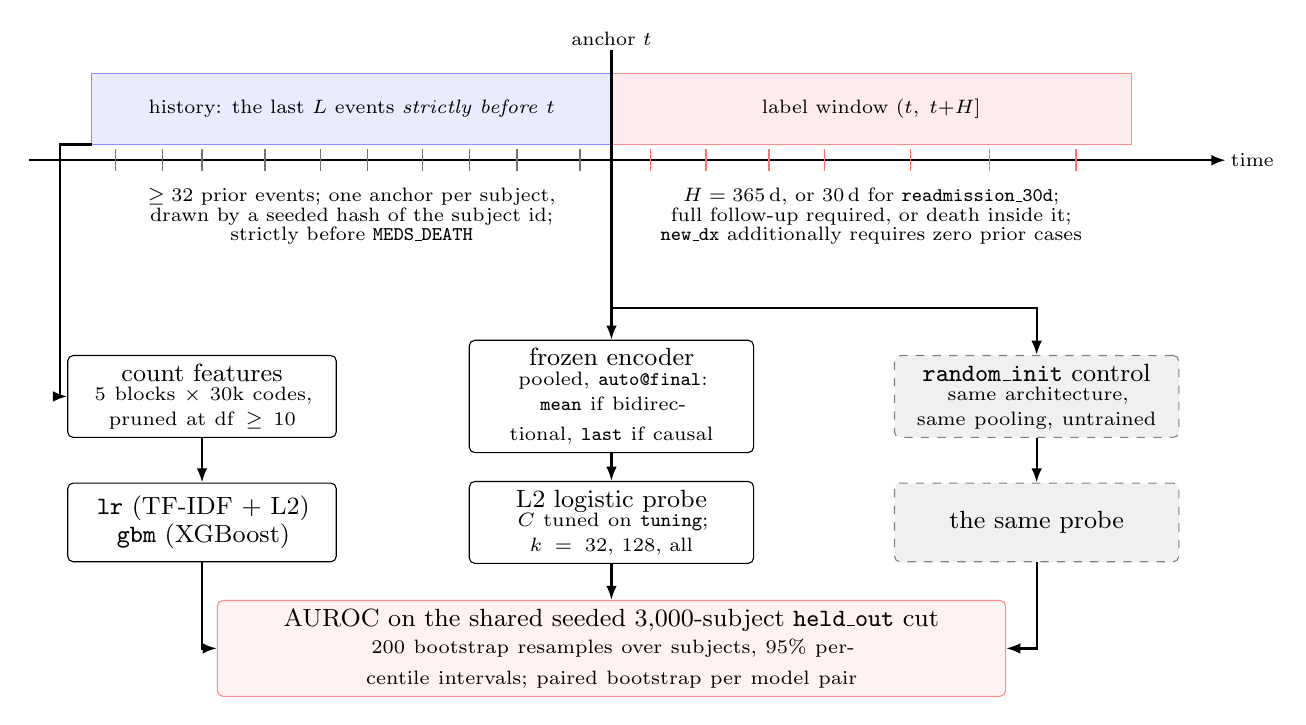
\begin{tikzpicture}[
  font=\small,
  fl/.style   = {-{Latex[length=1.8mm]}, thick},
  box/.style  = {draw, rounded corners=2pt, align=center, inner sep=3pt,
                 minimum height=10mm, fill=white},
  ctl/.style  = {box, fill=black!6, draw=black!50, dashed},
  res/.style  = {box, fill=red!5,  draw=red!45},
  lbl/.style  = {font=\scriptsize, inner sep=1.5pt},
]

% ================= timeline ============================================
\draw[fl] (0mm,0) -- (152mm,0) node[right, lbl] {time};

% history band
\fill[blue!8]  (8mm,2mm) rectangle (74mm,11mm);
\draw[blue!45] (8mm,2mm) rectangle (74mm,11mm);
\node[lbl, align=center] at (41mm,6.5mm)
  {history: the last $L$ events \emph{strictly before} $t$};

% label band
\fill[red!8]  (74mm,2mm) rectangle (140mm,11mm);
\draw[red!45] (74mm,2mm) rectangle (140mm,11mm);
\node[lbl, align=center] at (107mm,6.5mm) {label window $(t,\;t{+}H]$};

% anchor
\draw[very thick] (74mm,-4mm) -- (74mm,14mm);
\node[lbl, above] at (74mm,14mm) {anchor $t$};

% event ticks
\foreach \x in {11,17,22,30,37,43,50,56,62,70} {\draw[black!55] (\x mm,-1.4mm) -- (\x mm,1.4mm);}
\foreach \x in {79,86,94,101,112,122,133}      {\draw[red!55]   (\x mm,-1.4mm) -- (\x mm,1.4mm);}

% notes under the bands
\node[lbl, align=center, anchor=north] at (41mm,-3mm)
  {$\geq 32$ prior events; one anchor per subject,\\[-1pt]
   drawn by a seeded hash of the subject id;\\[-1pt]
   strictly before \texttt{MEDS\_DEATH}};
\node[lbl, align=center, anchor=north] at (107mm,-3mm)
  {$H = 365$\,d, or $30$\,d for \texttt{readmission\_30d};\\[-1pt]
   full follow-up required, or death inside it;\\[-1pt]
   \texttt{new\_dx} additionally requires zero prior cases};

% ================= models ==============================================
\node[box, text width=32mm] (feat) at (22mm,-30mm)
  {count features\\[-1pt]{\scriptsize 5 blocks $\times$ 30k codes,\\[-2pt]
   pruned at $\mathrm{df}\geq 10$}};
\node[box, text width=34mm] (enc)  at (74mm,-30mm)
  {frozen encoder\\[-1pt]{\scriptsize pooled, \texttt{auto@final}:\\[-2pt]
   \texttt{mean} if bidirectional, \texttt{last} if causal}};
\node[ctl, text width=34mm] (ri)   at (128mm,-30mm)
  {\texttt{random\_init} control\\[-1pt]{\scriptsize same architecture,\\[-2pt]
   same pooling, untrained}};

\node[box, text width=32mm] (base)  at (22mm,-46mm)
  {\texttt{lr} (TF-IDF $+$ L2)\\[-1pt]\texttt{gbm} (XGBoost)};
\node[box, text width=34mm] (probe) at (74mm,-46mm)
  {L2 logistic probe\\[-1pt]{\scriptsize $C$ tuned on \texttt{tuning};\\[-2pt]
   $k=32,\,128,\,\mathrm{all}$}};
\node[ctl, text width=34mm] (rprobe) at (128mm,-46mm)
  {the same probe};

\node[res, text width=98mm] (ci) at (74mm,-62mm)
  {AUROC on the shared seeded 3{,}000-subject \texttt{held\_out} cut\\[-1pt]
   {\scriptsize 200 bootstrap resamples over subjects, 95\% percentile intervals;
    paired bootstrap per model pair}};

% ================= edges ===============================================
\draw[fl] (8mm,2mm)  -- ++(-4mm,0) |- (feat.west);
\draw[fl] (74mm,-4mm) -- ++(0,-3mm) -- (enc.north);
\draw[fl] (enc.north) ++(0,4mm) -| (ri.north);
\draw[fl] (feat)  -- (base);
\draw[fl] (enc)   -- (probe);
\draw[fl] (ri)    -- (rprobe);
\draw[fl] (base.south)   |- (ci.west);
\draw[fl] (probe)        -- (ci);
\draw[fl] (rprobe.south) |- (ci.east);

\end{tikzpicture}
}
\caption{The evaluation protocol. Every model in a run --- count baselines,
frozen-encoder probes, and the untrained control --- is fit and scored on
identical anchors and identical rows, which is what makes the paired bootstrap
legitimate and stops a checkpoint from looking better on an easier subset.}
\label{fig:protocol}
\end{figure}

\subsection{Tasks}

Seven binary tasks, defined in ACES YAML from a shared predicate file so that
cohorts and label windows are declarative rather than implemented. Labels come
from the MEDS extract, never from the tensor cache --- the cache rolls rare
codes up to an ancestor, so \code{ICD9CM//25001} and \code{ICD9CM//25002} can
share an id there, and a label built on cache ids would not be the label its
name claims.

\begin{itemize}[leftmargin=*,itemsep=2pt,topsep=3pt]
\item \code{mortality\_365d} --- a \code{MEDS\_DEATH} event in
      $(t,\, t+365\text{d}]$.
\item \code{inpatient\_365d} --- an \code{ADMISSION//INPATIENT} in
      $(t,\, t+365\text{d}]$.
\item \code{readmission\_30d} --- anchored on an inpatient \emph{discharge};
      another inpatient admission in $(t,\, t+30\text{d}]$.
\item \code{new\_dx\_365d/\{ckd, copd, diabetes, heart\_failure\}} --- a first-ever
      occurrence of the condition in $(t,\, t+365\text{d}]$, restricted to
      subjects with \emph{zero} occurrences at or before the anchor. On
      DE-SynPUF the matchers are the ICD-9-CM prefixes 585, \{490, 491, 492,
      494, 496\} (asthma, 493, is deliberately excluded), 250 and 428
      respectively.
\end{itemize}

Every target window is \code{start\_inclusive: false, end\_inclusive: true},
i.e.\ the half-open interval $(t,\, t+H]$: the anchor event itself lies in
neither the history nor the label window.

\subsection{Anchors and leakage rules}

One anchor per subject. Candidate times are the subject's distinct event times,
filtered in order by: (i) bearing the task's anchor concept, where it has one
(only \code{readmission\_30d} does); (ii) at least 32 events strictly before;
(iii) strictly before \code{MEDS\_DEATH}, if the subject has one; and (iv)
either a full horizon of record afterwards or death inside the horizon ---
otherwise a negative label would be censoring, not a negative. Among survivors
the kept time is chosen by
\code{blake2b("anchor:\textless seed\textgreater:\textless subject\_id\textgreater")}
modulo the candidate count, so the draw is a pure function of $(\text{seed},
\text{subject\_id})$ and is independent of row order, shard count and library
version. The anchor seed is 20260903.

Everything a model sees passes through one choke point,
\code{EventSequenceDataset.windows\_at}, which binary-searches the cache's
\code{time\_min} with \code{side="left"}: an event whose timestamp equals the
anchor is excluded along with everything after it. Because anchors are strictly
before \code{MEDS\_DEATH} and history is strictly before the anchor, no event at
or after death can enter a history window. The test suite builds the cohort
twice, the second time with a \code{MEDS\_DEATH} inserted one day after each
held-out subject's anchor --- an event that flips \code{mortality\_365d} from 0
to 1 --- and asserts the count features and the encoder embeddings come out
bit-identical.

\subsection{Baselines, probes and controls}

\paragraph{Count-feature baselines.}
Five blocks of \code{vocab\_size} columns each --- $\log 1p$ counts over the
last 30 days, 365 days and all history, the most recent \code{value\_z} per
code, and a $\log 1p$ numeric-observation count --- giving roughly 150{,}000
columns, pruned to those nonzero in at least 10 \emph{training} rows
(103k--110k kept per task). \code{lr} is L2 logistic regression with $C$ tuned
on the \code{tuning} split over $(0.003, 0.01, 0.03, 0.1, 0.3, 1.0)$; sparse
inputs are scaled with a TF-IDF transform fit on \code{train} only.\footnote{An
earlier version scaled with \code{StandardScaler(with\_mean=False)}, which
divides each column by its own standard deviation; because most kept columns
are rare, this inflated their scale and forced the tuned $C$ to the low edge of
the grid on every task, capping \code{lr} at 0.55--0.59 AUROC --- below the
untrained control. The scaling was replaced and only \code{lr} refit; a
regression test reproduces the failure shape. This is recorded because the
uncorrected numbers appear in an earlier committed run.} \code{gbm} is XGBoost
with \code{tree\_method="hist"}, selected on \code{tuning} AUROC from three
settings, fit in a subprocess that never imports torch (both libraries ship
their own OpenMP runtime, and on macOS arm64 whichever loads second corrupts
the first).

\paragraph{Frozen-encoder probes.}
The encoder runs in \code{eval()} mode, fp32, under \code{no\_grad}, with no
masking, over the last \code{max\_len} events strictly before the anchor. The
pooled representation is fed to the same L2 logistic regression, $C$ tuned on
\code{tuning}. Nothing is fine-tuned, so a difference between two checkpoints is
a difference in the representation. Pooling is resolved per architecture:
\code{mean} over valid tokens for a bidirectional encoder, the final \emph{valid}
token for a causal one. This matters for cross-grid comparison: grid~1 probed
every cell at \code{cls\_mean@final}, while grids~2--5 and both scale grids use
the architecture-resolved default. A causal encoder's \code{[CLS]} row is a
function of the \code{[CLS]} parameter alone --- it sits at index 0 and attends
only to itself --- so half of its \code{cls\_mean} vector carries nothing.

\paragraph{Untrained controls.}
\code{random\_init} rebuilds the checkpoint's own architecture from its own
stored \code{model\_config} and skips \code{load\_state\_dict}, then runs the
identical probe at the identical pooling. A pretrained checkpoint that does not
beat its own untrained twin has not learned anything this probe can use. One
control is computed per (architecture, pooling) pair, not per cell.

\paragraph{Held-out cut and intervals.}
The evaluation split is capped at a seeded 3{,}000 subjects by the same
\code{blake2b} construction as the anchor draw, so a subject kept for one task
is kept for every task in which it appears; \code{train} and \code{tuning} are
untouched, so every model is still fit on the full training data. Metrics are
AUROC, AUPRC, Brier and calibration slope, each with a 95\% percentile
bootstrap over subjects at 200 resamples; resampled draws that are degenerate
for a ranking metric are dropped rather than imputed, and the surviving count is
reported. Every unordered model pair additionally receives a \emph{paired}
bootstrap on the same resampled index, so the interval on a difference is not
inflated by shared sampling variance.

\paragraph{Few-shot.}
For $k \in \{32, 128\}$, $k$ positives and $k$ negatives are drawn without
replacement from \code{train}, a probe is fit, and it is scored on the same
held-out split; five draws per (task, $k$, checkpoint). The tuning split is not
subsampled. \code{gbm} has no few-shot fits: it is fit out of process and its
returned object holds only the predictions for the matrix given at fit time, so
a few-shot refit would score against the wrong matrix.

\subsection{Cohort sizes}

Table~\ref{tab:cohorts} gives the funnel and prevalences before the
3{,}000-subject cut. Anchoring keeps 72{,}835 of 116{,}352 subjects for the
365-day tasks; the follow-up requirement removes more subjects (15{,}289) than
the history requirement (28{,}156) plus the death rule (72).

\begin{table}[t]
\centering\small
\caption{Cohort sizes and held-out prevalence for \code{desynpuf-s1}, before the
seeded 3{,}000-subject evaluation cut. \emph{Anchored} is subjects surviving the
anchor rule; \emph{labelled} is those remaining after the task's own inclusion
criterion (for \code{new\_dx}, having no prevalent case at or before the
anchor). After the cut every task's held-out set is exactly 3{,}000 subjects.}
\label{tab:cohorts}
\begin{tabular}{lrrrr}
\toprule
task & anchored & labelled & held-out $n$ & held-out rate \\
\midrule
\code{mortality\_365d}              & 72{,}835 & 72{,}835 & 7{,}358 & 0.0190 \\
\code{inpatient\_365d}              & 72{,}835 & 72{,}835 & 7{,}358 & 0.2098 \\
\code{readmission\_30d}             & 30{,}592 & 30{,}592 & 3{,}116 & 0.0501 \\
\code{new\_dx\_365d/diabetes}       & 72{,}835 & 49{,}293 & 4{,}939 & 0.2264 \\
\code{new\_dx\_365d/heart\_failure} & 72{,}835 & 61{,}024 & 6{,}164 & 0.1308 \\
\code{new\_dx\_365d/ckd}            & 72{,}835 & 63{,}999 & 6{,}487 & 0.0999 \\
\code{new\_dx\_365d/copd}           & 72{,}835 & 59{,}999 & 6{,}009 & 0.1340 \\
\bottomrule
\end{tabular}
\end{table}

%==============================================================================
\section{Experiments}
\label{sec:experiments}

\subsection{Pilot grids 1--4: 20 cells at a matched 48M-token budget}

Every cell in Table~\ref{tab:master} shares \code{configs/pretrain\_pilot.yaml}
(4-layer, 192-wide encoder; 2-layer, 96-wide predictor; SwiGLU; dropout 0.1),
the \code{desynpuf-s1} \code{train} split, 48{,}005{,}120 nominal token slots
(2{,}930 steps at batch 64 $\times$ \code{max\_len} 256), seed 0, and the same
seeded 3{,}000-subject held-out cut with 200 bootstrap resamples across all
seven tasks. Training was on an Apple M4 (MPS). At this budget a cell sees
$\approx$22.7M real events, or about 2.0 epochs of the 11.3M-event train split.
\emph{Gain} is a cell's mean AUROC across the seven tasks minus the same mean
for its own architecture- and pooling-matched \code{random\_init} control.

\begin{table}[p]
\centering\footnotesize
\caption{Pilot grids 1--4: held-out AUROC by task, all 20 trained cells and
their four controls, seed 0, 48M nominal token slots each. Sorted by mean AUROC
descending. \emph{Gain} is against the row's own control; it is ``---'' for the
count-feature baselines and for the control rows themselves. Grid-1 rows were
probed at \code{cls\_mean@final} and grid 2--4 rows at the architecture-resolved
default, so a grid-1 number is not directly comparable to a grid 2--4 number for
the same cell --- but every gain is against a control probed the same way as its
cell.}
\label{tab:master}
\resizebox{\textwidth}{!}{%
\begin{tabular}{llll rrrrrrr rr}
\toprule
cell & gr. & family & control
& \rotatebox{60}{inpatient} & \rotatebox{60}{mortality}
& \rotatebox{60}{ckd} & \rotatebox{60}{copd}
& \rotatebox{60}{diabetes} & \rotatebox{60}{heart fail.}
& \rotatebox{60}{readmiss.} & gain & mean \\
\midrule
\code{nextlatent\_h1416\_recon} & 4 & nextlatent & \code{@nextlat\_h1} & 0.7417 & 0.6332 & 0.7531 & 0.7487 & 0.7618 & 0.7642 & 0.6985 & $+$0.0923 & \best{0.7287} \\
\code{gbm}                      & --- & count & --- & 0.7440 & 0.5723 & 0.7654 & 0.7674 & 0.7721 & 0.7893 & 0.6724 & --- & 0.7261 \\
\code{ar}                       & 1 & ar & \code{@ar} & 0.7265 & 0.6060 & 0.7586 & 0.7552 & 0.7590 & 0.7437 & 0.6946 & $+$0.0445 & 0.7205 \\
\code{jepa\_recon\_notime}      & 3 & jepa$+$recon & \code{@jepa\_r\_nt} & 0.7043 & 0.6492 & 0.7116 & 0.7173 & 0.7538 & 0.7144 & 0.6714 & $+$0.0296 & 0.7031 \\
\code{jepa\_content\_recon}     & 2 & jepa$+$recon & \code{@jepa\_nt} & 0.7085 & 0.6265 & 0.7167 & 0.7141 & 0.7432 & 0.7154 & 0.6747 & $+$0.0263 & 0.6999 \\
\code{recon\_only}              & 3 & recon-only & \code{@jepa\_r\_nt} & 0.7077 & 0.6068 & 0.7193 & 0.7155 & 0.7441 & 0.7140 & 0.6854 & $+$0.0254 & 0.6990 \\
\code{recon\_only\_notime}      & 3 & recon-only & \code{@jepa\_r\_nt} & 0.7009 & 0.6173 & 0.7216 & 0.7117 & 0.7445 & 0.7069 & 0.6804 & $+$0.0240 & 0.6976 \\
\code{jepa\_notime}             & 2 & masked-span & \code{@jepa\_nt} & 0.6920 & 0.6332 & 0.7121 & 0.7167 & 0.7477 & 0.7089 & 0.6590 & $+$0.0221 & 0.6957 \\
\code{lr}                       & --- & count & --- & 0.7077 & 0.5537 & 0.7361 & 0.7258 & 0.7397 & 0.7438 & 0.6578 & --- & 0.6949 \\
\code{jepa\_recon}              & 2 & jepa$+$recon & \code{@jepa\_nt} & 0.7078 & 0.5954 & 0.7169 & 0.7112 & 0.7410 & 0.7122 & 0.6611 & $+$0.0187 & 0.6922 \\
\code{jepa\_recon\_nosig}       & 3 & jepa$+$recon & \code{@jepa\_r\_nt} & 0.6947 & 0.5923 & 0.7110 & 0.7138 & 0.7473 & 0.7092 & 0.6703 & $+$0.0177 & 0.6912 \\
\code{jepa\_ema\_nosig}         & 1 & masked-span & \code{@jepa\_ema} & 0.6927 & 0.6409 & 0.6968 & 0.6997 & 0.7379 & 0.7031 & 0.6597 & $+$0.0080 & 0.6901 \\
\code{jepa\_ema}                & 1 & masked-span & \code{@jepa\_ema} & 0.6798 & 0.6096 & 0.6944 & 0.7059 & 0.7418 & 0.7027 & 0.6460 & $+$0.0008 & 0.6829 \\
\code{random\_init@jepa\_ema}   & 1 & control & --- & 0.6850 & 0.6021 & 0.7005 & 0.6933 & 0.7264 & 0.7001 & 0.6675 & --- & 0.6821 \\
\code{jepa\_content}            & 2 & masked-span & \code{@jepa\_nt} & 0.6914 & 0.5998 & 0.6984 & 0.7010 & 0.7307 & 0.7019 & 0.6488 & $+$0.0081 & 0.6817 \\
\code{jepa\_shared\_sig}        & 1 & masked-span & \code{@jepa\_ema} & 0.6784 & 0.6573 & 0.6865 & 0.6948 & 0.7292 & 0.6955 & 0.6293 & $-$0.0006 & 0.6816 \\
\code{jepa\_ema\_future}        & 1 & masked-span & \code{@jepa\_ema} & 0.6819 & 0.5837 & 0.6943 & 0.7048 & 0.7382 & 0.7000 & 0.6612 & $-$0.0015 & 0.6806 \\
\code{jepa\_ema\_block}         & 1 & masked-span & \code{@jepa\_ema} & 0.6763 & 0.5859 & 0.6939 & 0.7035 & 0.7295 & 0.7097 & 0.6442 & $-$0.0046 & 0.6776 \\
\code{random\_init@ar}          & 1 & control & --- & 0.6751 & 0.6160 & 0.6940 & 0.6890 & 0.7211 & 0.6904 & 0.6464 & --- & 0.6760 \\
\code{jepa\_content\_future}    & 2 & masked-span & \code{@jepa\_nt} & 0.6784 & 0.5776 & 0.6947 & 0.6975 & 0.7277 & 0.6960 & 0.6528 & $+$0.0014 & 0.6750 \\
\code{random\_init@jepa\_notime}& 2/3 & control & --- & 0.6775 & 0.5699 & 0.6962 & 0.6961 & 0.7252 & 0.6882 & 0.6619 & --- & 0.6736 \\
\code{window\_30\_365\_recon}   & 4 & window & \code{@nextlat\_h1} & 0.6764 & 0.5944 & 0.6805 & 0.7054 & 0.7274 & 0.6951 & 0.6209 & $+$0.0350 & 0.6714 \\
\code{nextlatent\_h1416}        & 4 & nextlatent & \code{@nextlat\_h1} & 0.6687 & 0.6063 & 0.6886 & 0.6823 & 0.7198 & 0.6868 & 0.6401 & $+$0.0340 & 0.6704 \\
\code{window\_30\_365}          & 4 & window & \code{@nextlat\_h1} & 0.6725 & 0.5860 & 0.6859 & 0.7028 & 0.7279 & 0.6901 & 0.6259 & $+$0.0337 & 0.6702 \\
\code{nextlatent\_h1}           & 4 & nextlatent & \code{@nextlat\_h1} & 0.6601 & 0.6108 & 0.6829 & 0.6854 & 0.7198 & 0.6867 & 0.6225 & $+$0.0305 & 0.6669 \\
\code{random\_init@nextlat\_h1} & 4 & control & --- & 0.6469 & 0.5339 & 0.6580 & 0.6620 & 0.7100 & 0.6660 & 0.5781 & --- & 0.6364 \\
\bottomrule
\end{tabular}}
\end{table}

Two pairs of control rows land on numerically identical values.
\code{random\_init@jepa\_notime} and \code{random\_init@jepa\_recon\_notime} are
the same untrained $4\times192$ bidirectional encoder at seed 0 under
\code{mean@final} pooling; \code{random\_init@nextlatent\_h1} and grid 2's
\code{random\_init@ar\_last} are the same untrained causal encoder under
\code{last@final}. A probe reads only the embedding and the encoder, and
neither grid's reconstruction head nor its \code{notime} flag exists at
initialisation. Both pairs are computed independently in their own grids rather
than reused, so their agreeing is a determinism check.

\begin{figure}[t]
\centering

\includegraphics[width=0.95\textwidth]{pilot_desynpuf_auroc.png}
\caption{Held-out AUROC by task for \code{gbm}, \code{lr}, \code{ar}, the best
\code{jepa\_*} variant and their \code{random\_init} controls, at the 48M-token
pilot budget on DE-SynPUF sample 1.}
\label{fig:pilotauroc}
\end{figure}

\begin{figure}[t]
\centering
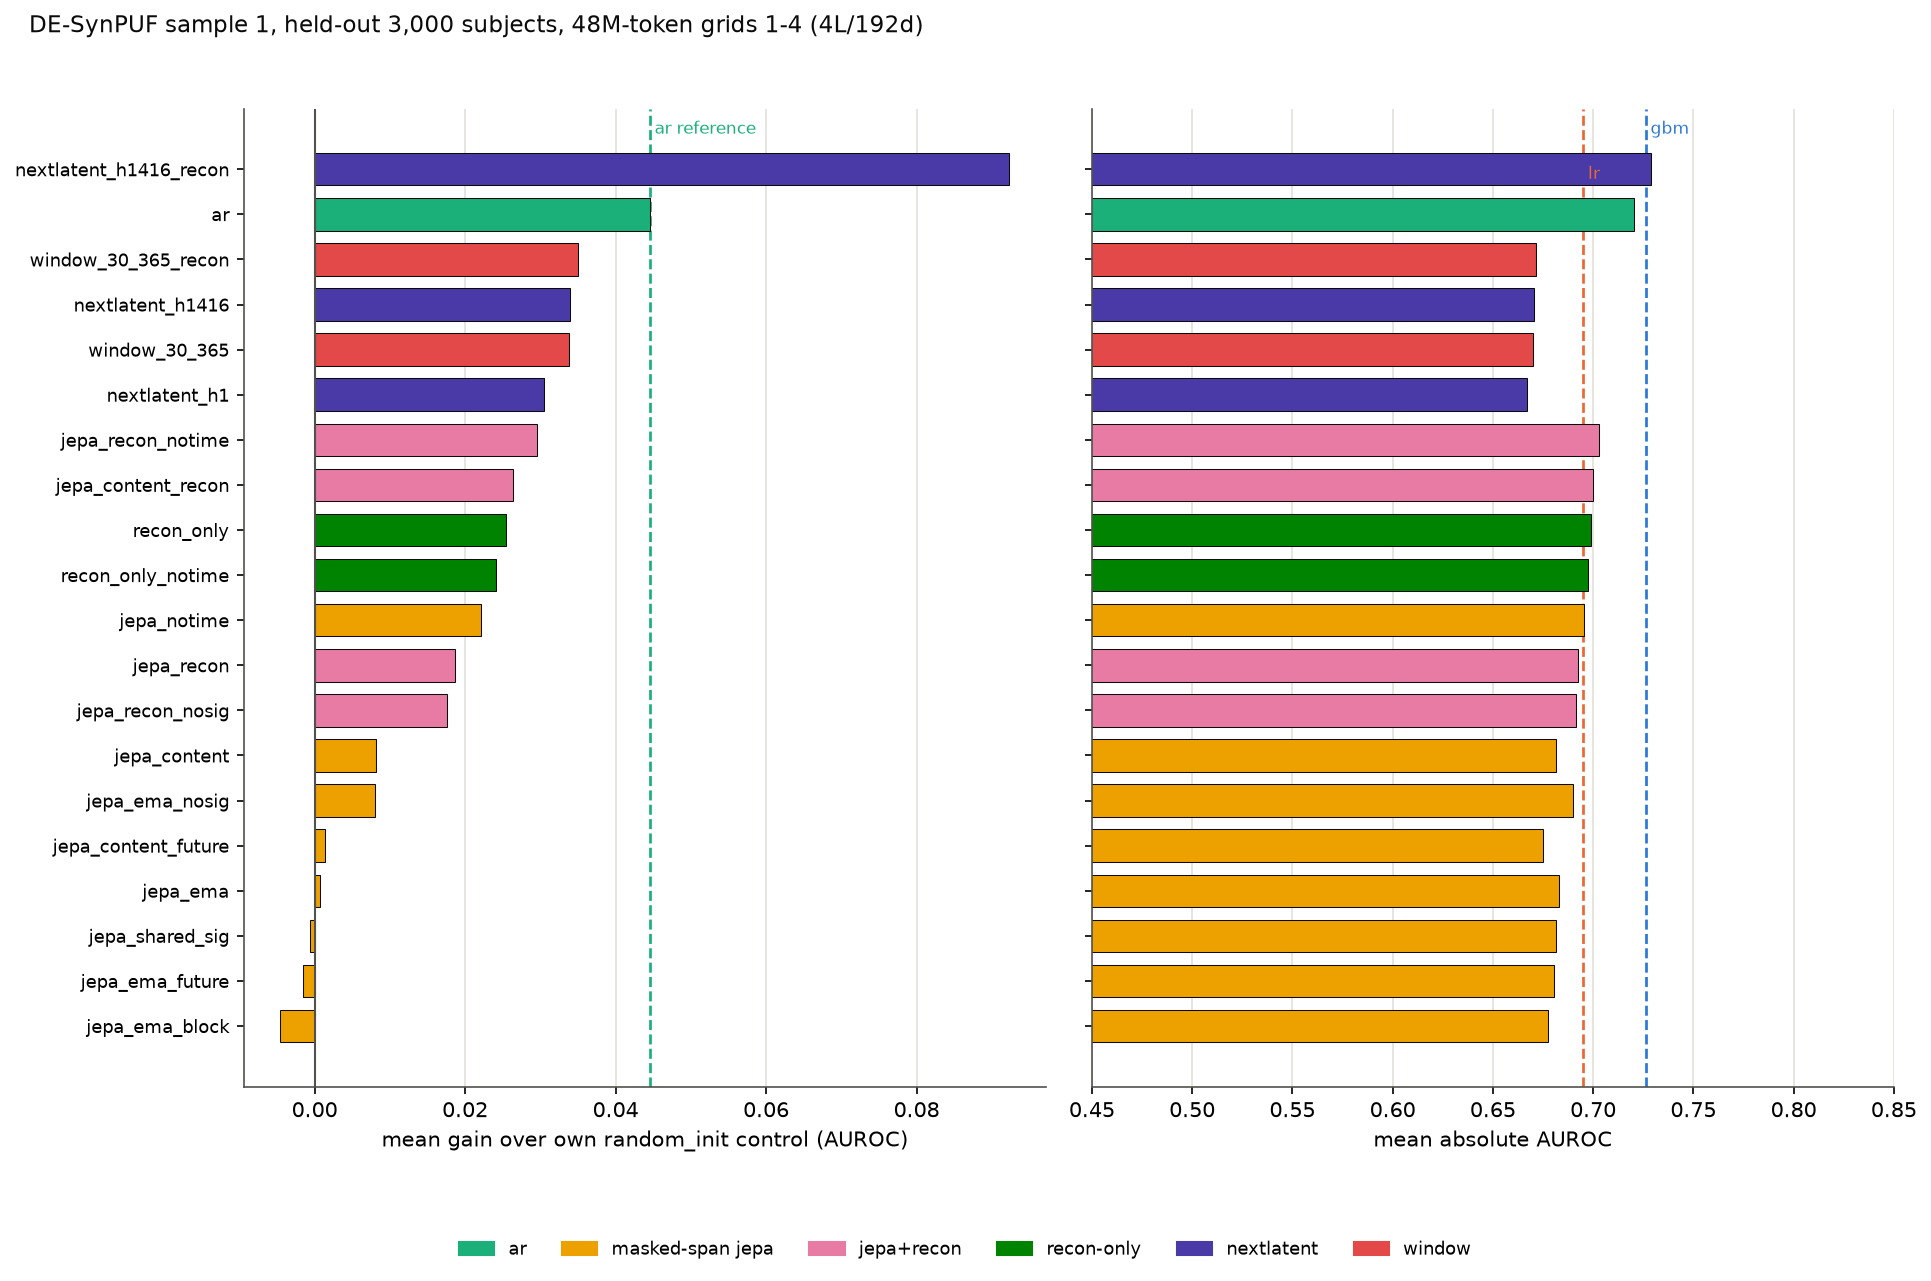
\includegraphics[width=0.95\textwidth]{pilot_grids_gain.png}
\caption{Mean gain over each cell's own \code{random\_init} control (left) and
mean absolute AUROC (right), by cell and objective family, across pilot grids
1--4. Regenerated by \code{scripts/plot\_grids.py}, which parses the four
committed \code{summary.md} tables directly.}
\label{fig:pilotgain}
\end{figure}

\paragraph{What each grid asked.}
Grid~1 asked whether JEPA beats AR at matched compute and whether either beats
an untrained control, sweeping target mode, SIGReg weight and masking mix one at
a time off \code{jepa\_ema}. Grid~2 asked whether four probe-independent
shortcuts explain grid~1's null result, closing a time-conditional prior, a
discarded-code-identity route and a context-copy route, with and without an
auxiliary code term. Grid~3 asked whether the latent smooth-$L_1$ term still
adds anything once code reconstruction is present: \code{recon\_only}, with
$\lambda_{\mathrm{pred}} = 0$ and no latent term at all, scores 0.6990, which is
0.0041 AUROC below \code{jepa\_recon\_notime} at 0.7031. Grid~4 asked whether
dense or window-pooled latent prediction transfers, alone and with code
supervision.

Two grid-2 rows are excluded from Table~\ref{tab:master}: \code{ar\_last} and
\code{jepa\_ema\_mean} train nothing --- they re-probe grid 1's checkpoints
under a different pooling, and including them would double-count two trained
cells as four.

\subsection{Diagnostics}
\label{sec:diagnostics}

Four measurements were taken on grid~1's checkpoints, before grid~2 was
designed against them. Each identifies a route by which the masked-span
objective can be satisfied without the encoder carrying anything a probe would
want. These were one-off measurements; unlike everything else in this paper
they do not have committed code in the repository, only their numbers and
prose definitions.

\begin{enumerate}[leftmargin=*,itemsep=3pt,topsep=3pt]
\item \textbf{The task is mostly a time-conditional prior.} A ridge map from the
      predictor's mask-token time features \emph{alone} reaches $R^2 = 0.58$ on
      the layer-normed targets; the trained predictor, which additionally sees
      the context, reaches $R^2 = 0.79$. Most of what the predictor produces is
      recoverable from ``what time is it'' without looking at the patient. The
      flag that closes this is \code{predictor.mask\_token\_time: false}, which
      reduces a mask token to the bare learned \code{[MASK]} embedding with
      rotary position at the target's original index as the only positional
      information left.
\item \textbf{The encoders discard code identity.} A linear probe recovering a
      token's own \code{code\_id} from the frozen encoder output scores top-1
      0.50 on the JEPA checkpoints, against \textbf{0.60 for the untrained
      encoder} and 0.71 for the AR one. Pretraining made this \emph{worse} than
      initialisation.
\item \textbf{Full-sequence targets admit a context-copy shortcut.} Without
      SIGReg the target embeddings are 45\% between-window variance, and a plain
      context-mean baseline reaches cosine 0.73 to the targets. The target
      encoder attends over the whole window, including the context the predictor
      was handed, so a target latent can contain what the predictor already has.
      The flag that closes this is \code{target.span\_only}.
\item \textbf{One diagnostic did not survive re-measurement.} Pooling was
      initially reported to be costing the causal arm 2.5--3.3 AUROC points
      (\code{last@final} against \code{cls\_mean@final} on the AR checkpoint).
      Re-scored on the full seven-task 3{,}000-subject held-out cut,
      \code{last} wins four tasks of seven, ranges from $-2.07$ to $+2.77$
      points, and averages $+0.17$. The pooling default was still changed, on
      the architectural argument given in Section~\ref{sec:eval}, but the
      \emph{size} of the effect is not what the diagnostic claimed. It is
      recorded here because the original figure appears in an earlier committed
      protocol document.
\end{enumerate}

Read against Table~\ref{tab:master}: closing the shortcuts moves the probe, but
not by much and not to where AR sits. \code{jepa\_notime} gains $+0.0221$ over
its control against \code{jepa\_ema}'s $+0.0008$; adding the code term takes
\code{jepa\_content\_recon} to $+0.0263$; but \code{recon\_only}, which has no
latent term at all, retains $+0.0254$ of that. A cell that closes a shortcut
and does not move the probe has said something --- that the shortcut was not
what was limiting the representation.

\subsection{Grid 5: seed replication at 48M tokens}

Grid~1's \code{ar} and grid~4's hybrid were retrained at seeds 1 and 2, same
base config, same budget, same cache, same held-out subset and bootstrap
protocol. Table~\ref{tab:seeds} gives the three-seed mean and standard
deviation per task.

\begin{table}[t]
\centering\small
\caption{Grid 5: three-seed mean $\pm$ population standard deviation and range
of held-out AUROC, at the 48M-token budget. Three-seed mean across the seven
tasks: \code{ar} 0.7234, hybrid 0.7279.}
\label{tab:seeds}
\resizebox{\textwidth}{!}{%
\begin{tabular}{lcccc}
\toprule
task & \code{ar} mean $\pm$ std & \code{ar} range & hybrid mean $\pm$ std & hybrid range \\
\midrule
\code{inpatient\_365d}              & $0.7417 \pm 0.0027$ & [0.7392, 0.7455] & $0.7445 \pm 0.0025$ & [0.7417, 0.7479] \\
\code{mortality\_365d}              & $0.6034 \pm 0.0061$ & [0.5951, 0.6094] & $0.6219 \pm 0.0109$ & [0.6072, 0.6332] \\
\code{new\_dx\_365d/ckd}            & $0.7480 \pm 0.0044$ & [0.7419, 0.7514] & $0.7525 \pm 0.0018$ & [0.7501, 0.7543] \\
\code{new\_dx\_365d/copd}           & $0.7604 \pm 0.0009$ & [0.7592, 0.7613] & $0.7515 \pm 0.0023$ & [0.7487, 0.7544] \\
\code{new\_dx\_365d/diabetes}       & $0.7618 \pm 0.0032$ & [0.7574, 0.7652] & $0.7643 \pm 0.0033$ & [0.7618, 0.7689] \\
\code{new\_dx\_365d/heart\_failure} & $0.7660 \pm 0.0069$ & [0.7562, 0.7714] & $0.7636 \pm 0.0041$ & [0.7584, 0.7683] \\
\code{readmission\_30d}             & $0.6824 \pm 0.0064$ & [0.6738, 0.6890] & $0.6969 \pm 0.0031$ & [0.6926, 0.6996] \\
\bottomrule
\end{tabular}}
\end{table}

The comparison this table supports is narrow. Per task, the \code{ar}-versus-hybrid
gap is \emph{smaller} than at least one of the two families' own seed ranges on
\code{inpatient\_365d}, \code{new\_dx\_365d/ckd}, \code{new\_dx\_365d/diabetes}
and \code{new\_dx\_365d/heart\_failure}. It exceeds both ranges on only three
tasks: \code{mortality\_365d}, \code{new\_dx\_365d/copd} and
\code{readmission\_30d}. On \code{copd} the sign is in \code{ar}'s favour.

\subsection{Few-shot}
\label{sec:fewshot}

Table~\ref{tab:fewshot} scores the six 1B checkpoints of
Section~\ref{sec:final1b} (\code{ar} and \code{hybrid\_final}, seeds 0--2
each), plus \code{lr}, at $k = 32$ and $k = 128$ ($k$ positives and $k$
negatives) as well as the full split, on the same \textbf{full held-out
split (11{,}708 subjects)} as Section~\ref{sec:final1b} --- superseding an
earlier few-shot run on the 48M-token pilot checkpoints and the
3{,}000-subject held-out subset
(\code{docs/experiments/2026-09-04-fewshot-desynpuf/}, dropped from this
paper; its numbers are unchanged in the repository for reference).
Averaged across the seven tasks: \code{lr} 0.6147 / 0.6391 / 0.6972;
\code{ar} 0.6131 / 0.6597 / 0.7239; \code{hybrid\_final} 0.6412 / 0.6872 /
0.7397. The \code{ar} and \code{hybrid\_final} $\pm$ values are the spread
over three \emph{training} seeds of each checkpoint's own mean over five
few-shot-sample seeds; \code{lr}'s is the spread over its five few-shot
seeds directly, since it has one model and no training-seed axis --- on this
full split \code{lr}'s $\pm$ is not negligible, up to $\pm0.0691$ at
$k{=}32$ on \code{new\_dx\_365d/copd}.

\begin{table}[t]
\centering\small
\caption{Few-shot held-out AUROC, full held-out split (11{,}708 subjects),
1B-token checkpoints. \code{gbm} is omitted: it has no few-shot fits in the
current evaluation path (Section~\ref{sec:eval}); its full-split numbers are
in Table~\ref{tab:final1bbaselines}.}
\label{tab:fewshot}
\resizebox{\textwidth}{!}{%
\begin{tabular}{lcccccc}
\toprule
task & \code{lr} $k{=}32$ & \code{lr} $k{=}128$ & \code{ar} $k{=}32$ & \code{ar} $k{=}128$ & hyb.\ $k{=}32$ & hyb.\ $k{=}128$ \\
\midrule
\code{inpatient\_365d}              & $0.5979 \pm 0.0390$ & $0.6613 \pm 0.0061$ & $0.6128 \pm 0.0040$ & $0.6772 \pm 0.0039$ & $0.6404 \pm 0.0048$ & $0.6959 \pm 0.0018$ \\
\code{mortality\_365d}              & $0.5295 \pm 0.0313$ & $0.5078 \pm 0.0381$ & $0.5369 \pm 0.0046$ & $0.5541 \pm 0.0036$ & $0.5414 \pm 0.0031$ & $0.5650 \pm 0.0032$ \\
\code{new\_dx\_365d/ckd}            & $0.6402 \pm 0.0569$ & $0.6795 \pm 0.0024$ & $0.6364 \pm 0.0027$ & $0.7056 \pm 0.0045$ & $0.6607 \pm 0.0026$ & $0.7307 \pm 0.0021$ \\
\code{new\_dx\_365d/copd}           & $0.6294 \pm 0.0691$ & $0.6722 \pm 0.0051$ & $0.6391 \pm 0.0068$ & $0.6976 \pm 0.0047$ & $0.6685 \pm 0.0030$ & $0.7192 \pm 0.0010$ \\
\code{new\_dx\_365d/diabetes}       & $0.6794 \pm 0.0183$ & $0.7007 \pm 0.0018$ & $0.6503 \pm 0.0046$ & $0.7049 \pm 0.0022$ & $0.6796 \pm 0.0018$ & $0.7289 \pm 0.0017$ \\
\code{new\_dx\_365d/heart\_failure} & $0.6588 \pm 0.0213$ & $0.6721 \pm 0.0066$ & $0.6488 \pm 0.0043$ & $0.6957 \pm 0.0039$ & $0.6816 \pm 0.0021$ & $0.7232 \pm 0.0017$ \\
\code{readmission\_30d}             & $0.5680 \pm 0.0284$ & $0.5799 \pm 0.0222$ & $0.5675 \pm 0.0147$ & $0.5827 \pm 0.0093$ & $0.6160 \pm 0.0064$ & $0.6477 \pm 0.0035$ \\
\bottomrule
\end{tabular}}
\end{table}

\begin{figure}[t]
\centering
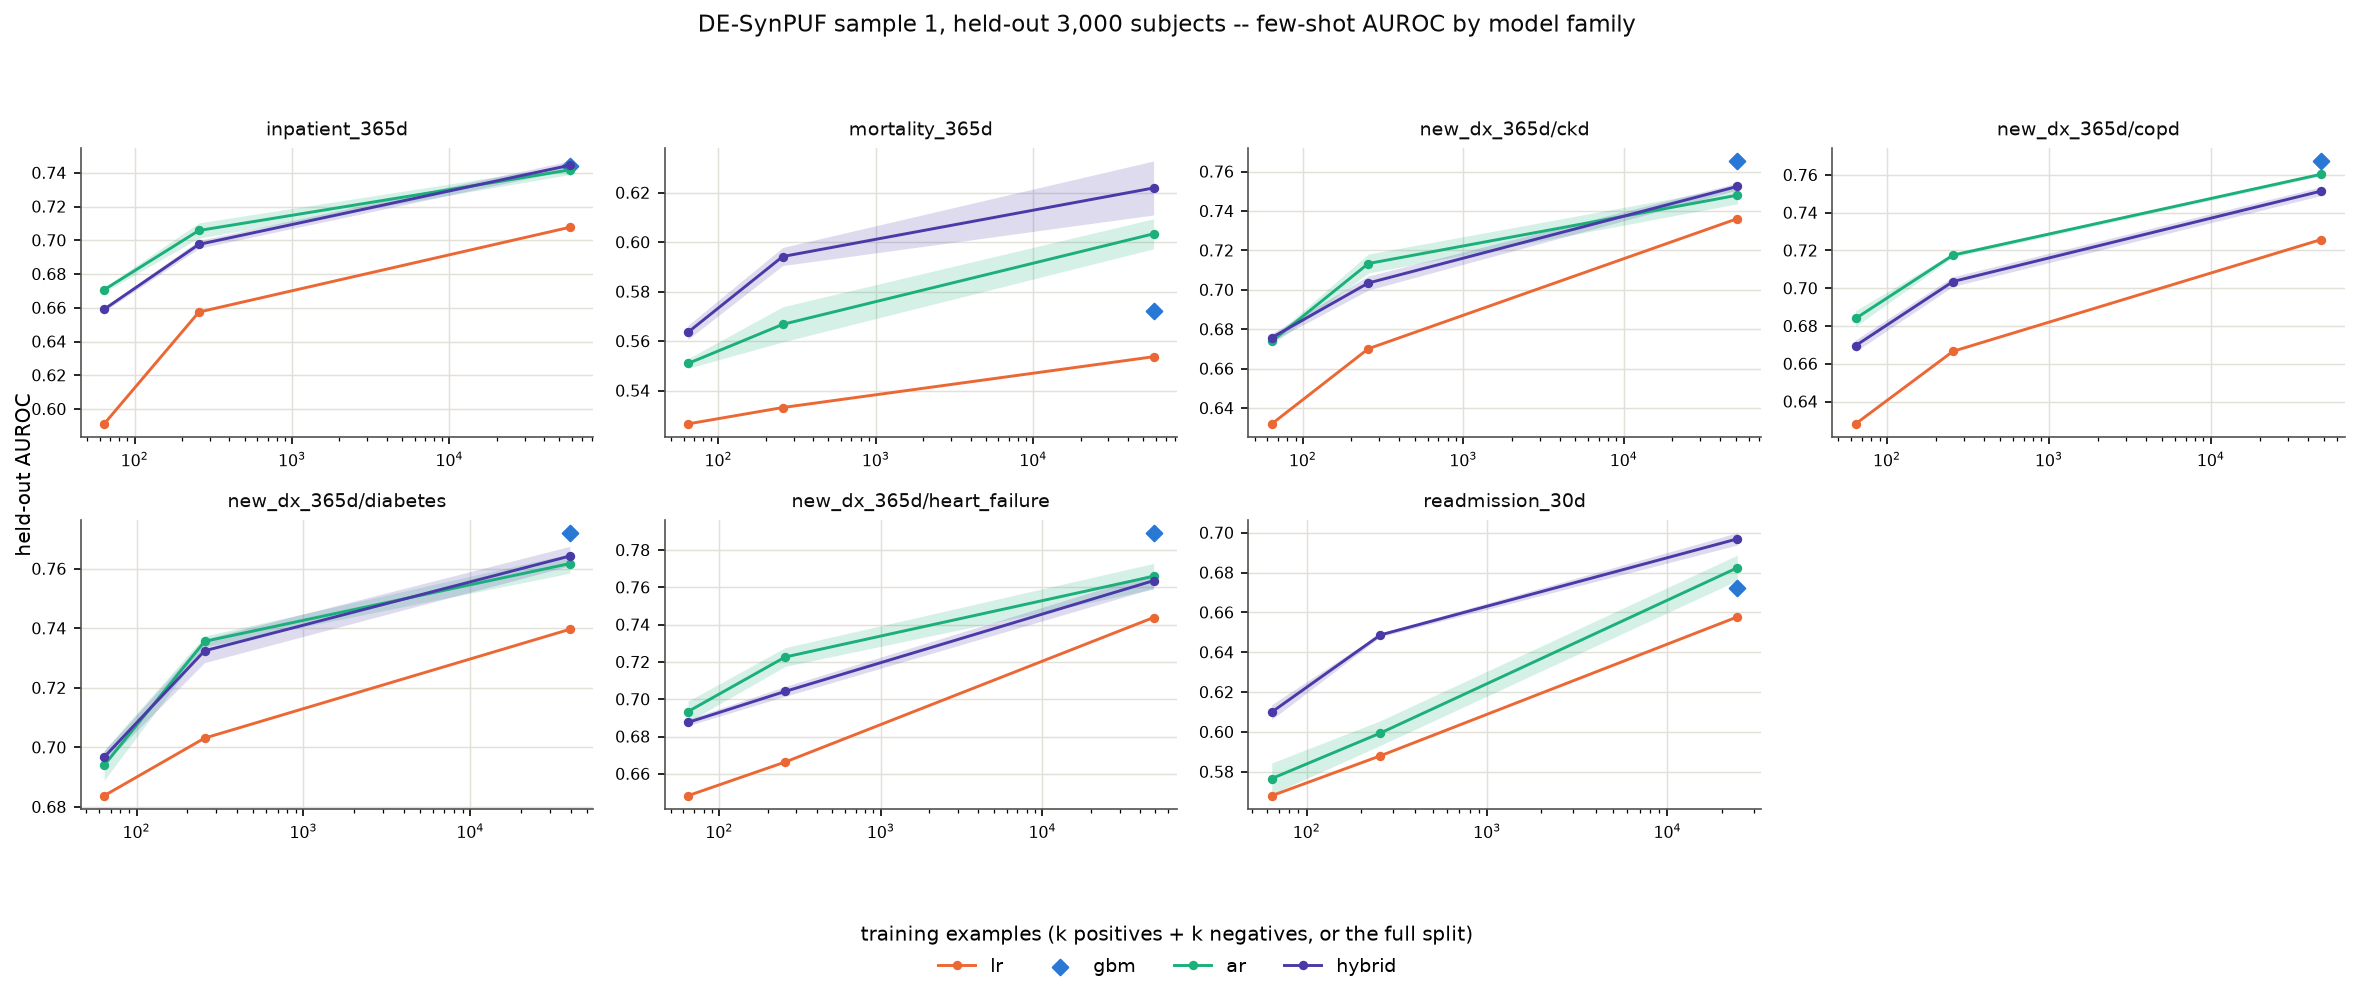
\includegraphics[width=\textwidth]{fewshot_desynpuf.png}
\caption{Held-out AUROC against few-shot training size, full held-out split,
one panel per task, one line per model family.}
\label{fig:fewshot}
\end{figure}

\code{hybrid\_final} is above \code{ar} and above \code{lr} at both $k{=}32$
and $k{=}128$ on every one of the seven tasks. \code{lr} is below both
encoder families at $k{=}128$ on every task; at $k{=}32$ \code{lr} is above
\code{ar} on four of seven tasks --- \code{new\_dx\_365d/ckd} (0.6402 vs.\
0.6364), \code{new\_dx\_365d/diabetes} (0.6794 vs.\ 0.6503),
\code{new\_dx\_365d/heart\_failure} (0.6588 vs.\ 0.6488) and
\code{readmission\_30d} (0.5680 vs.\ 0.5675) --- while remaining below
\code{hybrid\_final} on all seven. The largest \code{hybrid\_final}-over-\code{ar}
gap is on \code{readmission\_30d} at $k{=}128$ (0.6477 vs.\ 0.5827, $+0.0650$).

\subsection{Scaling to 200M and 1B tokens}
\label{sec:scale}

Two grids were run on an RTX 4060 (8\,GB) with
\code{configs/pretrain\_scale.yaml}: a 6-layer, 256-wide encoder with a 4-layer,
128-wide predictor, \code{max\_len} 512, batch 64, bf16, measured at roughly
33k tokens/s. The held-out subset, anchors, bootstrap settings and seven tasks
are identical to the pilot grids. Table~\ref{tab:scale} gives every trained cell
across all three budgets.

\begin{table}[t]
\centering\footnotesize
\caption{All trained cells across the three token budgets. The 48M rows are the
pilot grids (4-layer, 192-wide, Apple M4/MPS); the 200M and 1B rows are the
scale grids (6-layer, 256-wide, RTX 4060). Every row is seed 0 except the 1B
\code{ar} and hybrid rows, which are the 3-seed mean (seeds 0, 1, 2; see
Table~\ref{tab:seeds1b} for per-seed values, std and overlap). \code{gbm} and
\code{lr} do not depend on the encoder and are reused at every budget.}
\label{tab:scale}
\resizebox{\textwidth}{!}{%
\begin{tabular}{ll l rrrrrrr rr}
\toprule
cell & scale & family
& \rotatebox{60}{inpatient} & \rotatebox{60}{mortality}
& \rotatebox{60}{ckd} & \rotatebox{60}{copd}
& \rotatebox{60}{diabetes} & \rotatebox{60}{heart fail.}
& \rotatebox{60}{readmiss.} & mean & gain \\
\midrule
hybrid            & 48M  & nextlatent  & 0.7417 & 0.6332 & 0.7531 & 0.7487 & 0.7618 & 0.7642 & 0.6985 & 0.7287 & $+$0.0923 \\
\code{ar}         & 48M  & ar          & 0.7265 & 0.6060 & 0.7586 & 0.7552 & 0.7590 & 0.7437 & 0.6946 & 0.7205 & $+$0.0445 \\
\midrule
\code{gbm}        & ---  & count       & 0.7440 & 0.5723 & 0.7654 & 0.7674 & 0.7721 & 0.7893 & 0.6724 & 0.7261 & --- \\
\code{lr}         & ---  & count       & 0.7077 & 0.5537 & 0.7361 & 0.7258 & 0.7397 & 0.7438 & 0.6578 & 0.6949 & --- \\
\midrule
hybrid            & 200M & nextlatent  & 0.7511 & 0.5919 & 0.7761 & 0.7676 & 0.7729 & 0.7767 & 0.6930 & 0.7328 & $+$0.0781 \\
\code{ar}         & 200M & ar          & 0.7515 & 0.5946 & 0.7624 & 0.7747 & 0.7714 & 0.7908 & 0.6674 & 0.7304 & $+$0.0757 \\
\code{recon\_only}& 200M & recon-only  & 0.7326 & 0.6508 & 0.7336 & 0.7242 & 0.7568 & 0.7453 & 0.6894 & 0.7190 & $+$0.0448 \\
\code{jepa\_ema}  & 200M & masked-span & 0.6948 & 0.6413 & 0.7108 & 0.7189 & 0.7499 & 0.7159 & 0.6580 & 0.6985 & $+$0.0243 \\
\midrule
hybrid (3-seed)   & 1B   & nextlatent  & 0.7533 & 0.5866 & 0.7737 & 0.7780 & 0.7783 & 0.7987 & 0.6853 & \best{0.7363} & $+$0.0816 \\
\code{ar} (3-seed)& 1B   & ar          & 0.7452 & 0.5997 & 0.7584 & 0.7674 & 0.7615 & 0.7796 & 0.6637 & 0.7251 & $+$0.0704 \\
\bottomrule
\end{tabular}}
\end{table}

\code{random\_init@ar} is 0.6547 mean AUROC at both 200M and 1B (the same
untrained $6\times256$ causal encoder at the same seed);
\code{random\_init@hybrid} at 1B is numerically identical to it, for the same
reason the pilot control pairs agree. \code{random\_init@jepa\_ema} at 200M is
0.6742.

The \code{ar} row at 1B was re-evaluated after a fix to the evaluation
harness. Before commit \code{8721a62}, a checkpoint model's embedding cache was
keyed on its display name alone, so a second grid whose cell was also named
\code{ar} shared one cache file with the 200M grid's \code{ar} and would have
silently reported that grid's numbers. The cache key now includes a content
fingerprint of the checkpoint file itself.

\begin{table}[t]
\centering\small
\caption{\code{ar} against the hybrid across the three token budgets, mean
AUROC and the \code{readmission\_30d} column. 48M and 200M rows are seed 0;
the 1B row is the 3-seed mean (Table~\ref{tab:seeds1b}).}
\label{tab:scaling}
\begin{tabular}{lcccc}
\toprule
tokens & \code{ar} mean & \code{ar} readmission & hybrid mean & hybrid readmission \\
\midrule
48M  & 0.7205 & 0.6946 & 0.7287 & 0.6985 \\
200M & 0.7304 & 0.6674 & 0.7328 & 0.6930 \\
1B (3-seed) & 0.7251 & 0.6637 & \best{0.7363} & \best{0.6853} \\
\bottomrule
\end{tabular}
\end{table}

\begin{figure}[t]
\centering

\includegraphics[width=\textwidth]{scale_desynpuf.png}
\caption{Left: mean AUROC against token budget (log $x$) for \code{ar}, the
hybrid, \code{recon\_only} and \code{jepa\_ema} on the 3{,}000-subject
held-out subset (circles), with \code{gbm} as a horizontal reference; the
subset 1B \code{ar}/hybrid points are 3-seed means with a min-max error bar.
The diamonds at 1B are the full-held-out-split (Section~\ref{sec:final1b})
3-seed means for \code{ar} and \code{hybrid\_final}, offset in $x$ so they do
not overlap the subset circles. Right: per-task AUROC at 1B tokens on the
full held-out split, \code{ar} against \code{hybrid\_final}, paired bars,
each a 3-seed mean with a min-max whisker.}
\label{fig:scale}
\end{figure}

\paragraph{Measured behaviour across budgets.}
\code{ar} goes 0.7205 $\to$ 0.7304 $\to$ 0.7251 (1B a 3-seed mean). It does
not improve from 200M to 1B ($-0.0053$) and drops on six of seven tasks over
that step --- every task but \code{mortality\_365d} ($0.5946 \to 0.5997$,
$+0.0051$): \code{inpatient} $0.7515 \to 0.7452$, \code{ckd}
$0.7624 \to 0.7584$, \code{copd} $0.7747 \to 0.7674$, \code{diabetes}
$0.7714 \to 0.7615$, \code{heart\_failure} $0.7908 \to 0.7796$, and
\code{readmission\_30d} $0.6674 \to 0.6637$. The hybrid improves at every
step: 0.7287 $\to$ 0.7328 $\to$ 0.7363 (1B a 3-seed mean), that is $+0.0041$
then $+0.0035$. At 1B (3-seed means) the hybrid leads \code{ar} on six of
seven tasks --- every task but \code{mortality\_365d} --- by 0.81 to 2.16
AUROC points (\code{inpatient} $+0.81$, \code{ckd} $+1.53$, \code{copd}
$+1.05$, \code{diabetes} $+1.68$, \code{heart\_failure} $+1.92$,
\code{readmission} $+2.16$); \code{ar} leads on \code{mortality\_365d} by 1.31
points. The hybrid at 1B (0.7363, 3-seed mean) is the highest mean AUROC of
any cell in the table, above \code{gbm} at 0.7261 and \code{lr} at 0.6949.
\code{recon\_only} and \code{jepa\_ema} were run through 200M only.

\subsection{Seed replication at 1B}
\label{sec:seeds1b}

A seed-replication grid at the 1B budget (\code{scale1b-seeds-desynpuf}: seeds 1
and 2 for both \code{ar} and the hybrid, four cells) has completed, giving
three seeds (0, 1, 2) per cell. Table~\ref{tab:seeds1b} gives every per-seed
value plus the per-task mean and sample standard deviation ($n{=}3$) for
\code{ar} and the hybrid.

\begin{table}[t]
\centering\small
\caption{1B seed replication, complete: three seeds per cell for \code{ar} and
the hybrid. \code{std} is the sample standard deviation across the three
seeds ($n{=}3$). Seed 0 rows repeat Table~\ref{tab:scale}'s single-seed 1B
values; the mean rows repeat Table~\ref{tab:scale}'s 3-seed 1B values.}
\label{tab:seeds1b}
\resizebox{\textwidth}{!}{%
\begin{tabular}{ll rrrrrrr r}
\toprule
cell & seed
& \rotatebox{60}{inpatient} & \rotatebox{60}{mortality}
& \rotatebox{60}{ckd} & \rotatebox{60}{copd}
& \rotatebox{60}{diabetes} & \rotatebox{60}{heart fail.}
& \rotatebox{60}{readmiss.} & mean \\
\midrule
\code{ar} & 0 & 0.7506 & 0.6028 & 0.7586 & 0.7629 & 0.7618 & 0.7804 & 0.6490 & 0.7237 \\
\code{ar} & 1 & 0.7410 & 0.6031 & 0.7584 & 0.7738 & 0.7639 & 0.7796 & 0.6742 & 0.7277 \\
\code{ar} & 2 & 0.7441 & 0.5933 & 0.7581 & 0.7656 & 0.7589 & 0.7787 & 0.6679 & 0.7238 \\
\code{ar} & mean & 0.7452 & 0.5997 & 0.7584 & 0.7674 & 0.7615 & 0.7796 & 0.6637 & \best{0.7251} \\
\code{ar} & std & 0.0049 & 0.0056 & 0.0003 & 0.0057 & 0.0025 & 0.0009 & 0.0131 & --- \\
\midrule
hybrid & 0 & 0.7553 & 0.5767 & 0.7741 & 0.7781 & 0.7779 & 0.7997 & 0.6874 & 0.7356 \\
hybrid & 1 & 0.7491 & 0.5862 & 0.7717 & 0.7798 & 0.7787 & 0.8015 & 0.6846 & 0.7359 \\
hybrid & 2 & 0.7556 & 0.5969 & 0.7752 & 0.7760 & 0.7784 & 0.7950 & 0.6840 & 0.7373 \\
hybrid & mean & 0.7533 & 0.5866 & 0.7737 & 0.7780 & 0.7783 & 0.7987 & 0.6853 & \best{0.7363} \\
hybrid & std & 0.0037 & 0.0101 & 0.0018 & 0.0019 & 0.0004 & 0.0034 & 0.0018 & --- \\
\bottomrule
\end{tabular}}
\end{table}

\paragraph{Per-task overlap.} Comparing the min-max range across the three
seeds, \code{ar} and the hybrid do not overlap on \code{ckd} (\code{ar}
$0.7581$--$0.7586$ vs.\ hybrid $0.7717$--$0.7752$), \code{diabetes}
($0.7589$--$0.7639$ vs.\ $0.7779$--$0.7787$), \code{heart\_failure}
($0.7787$--$0.7804$ vs.\ $0.7950$--$0.8015$) and \code{readmission\_30d}
($0.6490$--$0.6742$ vs.\ $0.6840$--$0.6874$). They overlap on
\code{inpatient\_365d} ($0.7410$--$0.7506$ vs.\ $0.7491$--$0.7556$) and
\code{mortality\_365d} ($0.5933$--$0.6031$ vs.\ $0.5767$--$0.5969$).
\code{copd} does not overlap by the same min-max definition, but by the
smallest margin of any non-overlapping task: \code{ar}'s maximum ($0.7738$)
sits $0.0022$ below the hybrid's minimum ($0.7760$).

The largest hybrid-over-\code{ar} margin at 1B, on \code{readmission\_30d}
(Table~\ref{tab:scale}, $+2.16$ points on the 3-seed means), is also a task
whose seed ranges do not overlap between the two objectives: every one of
\code{ar}'s three seeds (0.6490, 0.6742, 0.6679) is below every one of the
hybrid's three seeds (0.6874, 0.6846, 0.6840). \code{ar}'s within-family seed
spread on this task (0.0131 std, the largest of any task for either
objective) is therefore smaller than its gap to the hybrid, not comparable to
it as the single-seed-1 replicate suggested.


\subsection{Model size and hybrid ablations}
\label{sec:ablate2}

A third grid (\code{ablate2-desynpuf}, 18 rows) asks two questions the 200M/1B
grids above cannot: does the hybrid's lead over \code{ar} depend on model
size, and which of the hybrid's own knobs (target mode, SIGReg weight,
horizon set, reconstruction weight) matter? It trains \code{ar} and the
hybrid at three sizes --- small (4-layer, 192-wide, 4 heads), base (6-layer,
256-wide, the \code{scale} shape, re-scored from
\code{runs/scale-desynpuf/\{ar,hybrid\}/final.pt} rather than retrained), and
large (8-layer, 384-wide, 6 heads) --- each at 200M nominal token slots, and
sweeps four single-knob variants of the base-size hybrid. Every trained cell
runs at two seeds (1 and 2); the re-scored base cells carry only their
original seed 0. Unlike every grid above, evaluation here covers the full
held-out split (11{,}708 subjects, not the seeded 3{,}000-subject subset), so
these numbers are not directly comparable to Tables~\ref{tab:master}
and~\ref{tab:scale}. Full protocol and per-task tables are in
\code{docs/experiments/ABLATION\_RESULTS.md}.

\begin{table}[t]
\centering\footnotesize
\caption{\code{ar} vs.\ hybrid at three sizes, full held-out split (11{,}708
subjects), 200M nominal token slots per cell. Small and large rows are 2-seed
means; base rows are seed 0 only (re-scored \code{scale-desynpuf}
checkpoints). Trainable parameter counts are computed from each model's
actual construction (Appendix~\ref{app:repro}'s configs plus the grid's
per-cell overrides), not estimated. \emph{mean-6} excludes
\code{mortality\_365d}; \emph{mean-7} includes it.}
\label{tab:ablate2size}
\begin{tabular}{llr rr}
\toprule
size & family & params & mean-6 & mean-7 \\
\midrule
small & \code{ar}     & 7.70M & 0.7460 & 0.7259 \\
small & hybrid         & 8.01M & \best{0.7539} & \best{0.7364} \\
base (seed 0) & \code{ar}   & 12.7M & 0.7507 & 0.7315 \\
base (seed 0) & hybrid       & 13.2M & \best{0.7554} & \best{0.7345} \\
large & \code{ar}     & 26.2M & 0.7540 & 0.7336 \\
large & hybrid         & 27.4M & \best{0.7595} & \best{0.7382} \\
\bottomrule
\end{tabular}
\end{table}

\begin{table}[t]
\centering\footnotesize
\caption{Base-size (6-layer, 256-wide) hybrid-knob comparison, mean AUROC
across the six non-mortality tasks. \emph{default} is \code{hybrid\_base\_s0}
(seed 0 only); the other four rows are 2-seed means. \emph{seed spread} is the
per-task $|s1 - s2|$ averaged over the six tasks.}
\label{tab:ablate2knobs}
\begin{tabular}{lrr}
\toprule
knob & mean-6 & seed spread \\
\midrule
default (\code{lambda\_recon}=0.1, EMA target, horizons [1,4,16]) & 0.7554 & --- \\
shared target (instead of EMA) & 0.7510 & 0.0029 \\
no SIGReg (\code{lambda\_sigreg}=0) & \best{0.7615} & 0.0039 \\
horizon [1] only (instead of [1,4,16]) & 0.7512 & 0.0020 \\
\code{lambda\_recon}=0.3 (instead of 0.1) & 0.7593 & 0.0046 \\
\bottomrule
\end{tabular}
\end{table}

\begin{figure}[t]
\centering
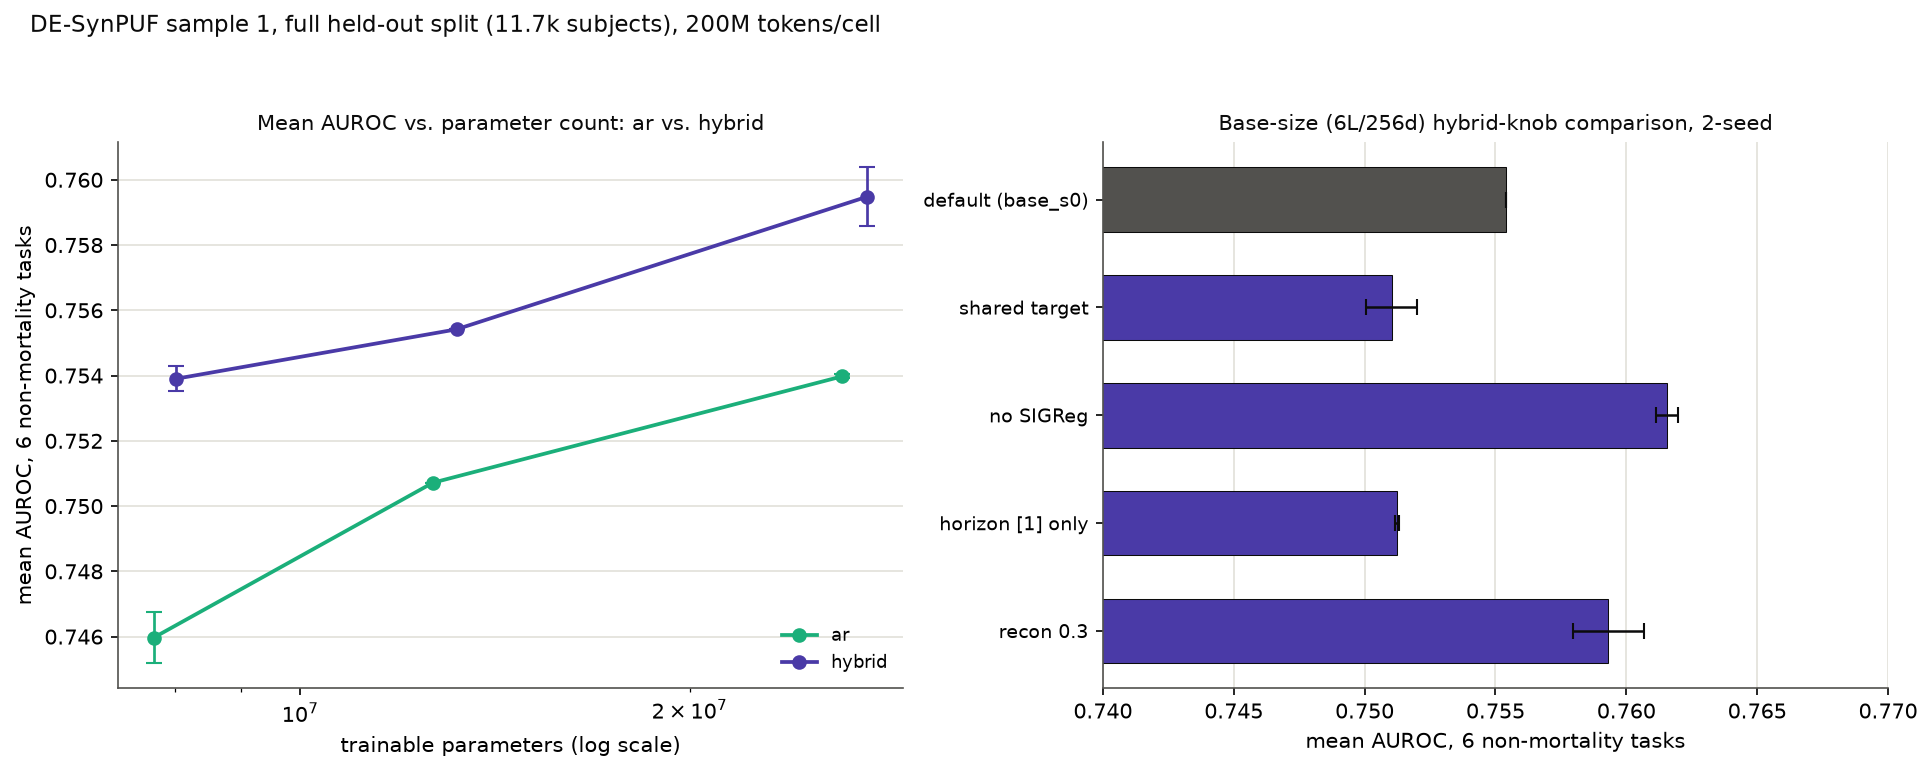
\includegraphics[width=\textwidth]{ablate2_desynpuf.png}
\caption{Left: mean AUROC across the six non-mortality tasks against
trainable parameter count (log $x$) for \code{ar} and the hybrid across the
three sizes, with 2-seed min-max error bars (none at base, seed 0 only).
Right: the base-size hybrid-knob comparison as horizontal bars with 2-seed
min-max whiskers (none for the default row). Regenerated by
\code{scripts/plot\_ablate2.py}, which builds each model from its config
overrides to compute the parameter counts rather than reading a hand-typed
estimate.}
\label{fig:ablate2}
\end{figure}

\paragraph{Size.} The hybrid leads \code{ar} on the 6-task mean at every
size: $+0.0079$ (small), $+0.0047$ (base), $+0.0055$ (large). The gap does
not close as size increases --- base's gap is the smallest of the three, and
large's is larger than base's.

\paragraph{Knobs.} No-SIGReg is the best knob at both seeds individually
(0.7620 at seed 1, 0.7611 at seed 2), ahead of the other three variants at
both seeds. Horizon-[1]-only (0.7512) and shared-target (0.7510) are the
worst knobs, both below the 0.7554 default. \code{lambda\_recon}=0.3 (0.7593)
is within 0.0039 of the 0.1 default, inside the 0.0020--0.0046 seed spread
measured among these four knobs.

\paragraph{Decision.} Section~\ref{sec:roadmap} adopts a new default
configuration (\code{configs/pretrain\_default.yaml}) from this result: the
hybrid objective, causal encoder, horizons $[1, 4, 16]$,
$\lambda_{\mathrm{recon}} = 0.1$, and $\lambda_{\mathrm{sig}} = 0$ --- SIGReg
dropped, per the no-SIGReg result above. The target encoder is EMA, not the
frozen AR teacher of Section~\ref{sec:ablate3}: Section~\ref{sec:ablate4}
finds the two gains do not stack, so there is no accuracy reason to prefer
the frozen teacher, and EMA is the self-contained choice.

\paragraph{Caveats.} The base-size default row is one seed, so every
size/knob comparison against it is a 2-seed-vs-1-seed comparison, not
2-seed-vs-2-seed. 200M nominal token slots, DE-SynPUF only. Differences among
the base-size hybrid knobs are 0.3--0.7 points (mean-6, vs.\ the default)
against a seed spread of about 0.3--0.5 points among those same knobs.

\subsection{Teachers and code-embedding initialization}
\label{sec:ablate3}

A fourth grid (\code{ablate3-desynpuf}, complete) asks two further questions
at the same base size, budget and full-held-out protocol as
Section~\ref{sec:ablate2}: can a frozen pretrained teacher replace EMA as the
target encoder, and does initializing the code embedding table from text
descriptions of each code help either objective? Five configurations, two
seeds each. \code{hybrid\_frozen\_ar} sets \code{model.target\_mode: frozen}
and loads the target embedding and encoder from the 1B-token
\code{scale1b-desynpuf} \code{ar} checkpoint, never updating it.
\code{hybrid\_frozen\_ar\_init} additionally initializes the \emph{student}
from that checkpoint (\code{model.init\_from}), separating the value of a
pretrained target from the value of a pretrained student.
\code{hybrid\_textinit} and \code{ar\_textinit} replace the $\mathcal{N}(0,
0.02)$ code table with projected sentence embeddings of each code's
description under both objectives; \code{hybrid\_textinit\_frozen} freezes
that table.

\begin{table}[t]
\centering\footnotesize
\caption{\code{ablate3-desynpuf}, full held-out split, 200M nominal token
slots per cell, 2-seed means. \emph{mean-6} excludes
\code{mortality\_365d}; \emph{mean-7} includes it; \emph{seed spread} is the
per-task $|s1-s2|$ averaged over the six non-mortality tasks. References:
\code{hybrid\_base\_s0} (EMA default, seed 0) and \code{ar\_base\_s0} (seed
0) are Table~\ref{tab:ablate2size}'s base row; \code{hybrid\_nosig} is
Table~\ref{tab:ablate2knobs}'s no-SIGReg row.}
\label{tab:ablate3}
\begin{tabular}{lrrr}
\toprule
config & mean-6 & mean-7 & seed spread \\
\midrule
\code{hybrid\_frozen\_ar} & \best{0.7615} & 0.7404 & 0.0036 \\
\code{hybrid\_frozen\_ar\_init} & 0.7559 & 0.7359 & 0.0013 \\
\code{hybrid\_textinit} & 0.7561 & 0.7367 & 0.0022 \\
\code{hybrid\_textinit\_frozen} & 0.7546 & 0.7344 & 0.0053 \\
\code{ar\_textinit} & 0.7490 & 0.7283 & 0.0052 \\
\midrule
\code{hybrid\_base\_s0} (EMA default) & 0.7554 & 0.7345 & --- \\
\code{hybrid\_nosig} (no SIGReg) & 0.7615 & --- & --- \\
\code{ar\_base\_s0} & 0.7507 & 0.7315 & --- \\
\bottomrule
\end{tabular}
\end{table}

\paragraph{Findings.} The frozen AR teacher gains $+0.6$ (mean-6) over the
EMA default (0.7615 vs.\ 0.7554) --- the same value, and the same gain, as
the no-SIGReg result in Section~\ref{sec:ablate2}. Initializing the student
from the same checkpoint removes the gain (\code{hybrid\_frozen\_ar\_init}
0.7559 vs.\ 0.7554, $+0.0005$): the frozen-teacher gain is a property of the
target, not of a pretrained student. Text-initialized code embeddings are
neutral for both objectives (\code{hybrid\_textinit} $+0.0007$ over the EMA
default, \code{ar\_textinit} $-0.0017$ against \code{ar\_base\_s0}, both
inside the 0.0022--0.0052 seed spread on these cells). Freezing the text
table costs 0.1 (0.7561 vs.\ 0.7546) while removing 58\% of the trainable
parameters --- the code table is 7{,}680{,}000 of the base-size hybrid's
13{,}208{,}336 trainable parameters; freezing it leaves 5{,}528{,}336
trainable.

\subsection{Grid 4: do the no-SIGReg and frozen-teacher gains stack?}
\label{sec:ablate4}

A fifth grid (\code{ablate4-desynpuf}, complete) puts the two +0.6-point
knobs from Sections~\ref{sec:ablate2} and~\ref{sec:ablate3} --- dropping
SIGReg, and a frozen 1B-token AR checkpoint as the target encoder --- in the
same cell, \code{hybrid\_nosig\_frozen}, at two seeds, same base size, budget
and full-held-out protocol as the two grids above.

\begin{table}[h]
\centering\small
\caption{\code{ablate4-desynpuf}, full held-out split, 200M nominal token
slots per cell, 2-seed mean-of-6 (excludes \code{mortality\_365d}).}
\label{tab:ablate4}
\begin{tabular}{lr}
\toprule
config & mean-6 \\
\midrule
\code{hybrid\_nosig} (no SIGReg alone, Grid 2) & 0.7615 \\
\code{hybrid\_frozen\_ar} (frozen teacher alone, Grid 3) & 0.7615 \\
\code{hybrid\_nosig\_frozen} (both, this grid) & \best{0.7625} \\
\code{hybrid\_base\_s0} (EMA default, seed 0) & 0.7554 \\
\bottomrule
\end{tabular}
\end{table}

\paragraph{Finding.} The two effects do not stack.
\code{hybrid\_nosig\_frozen}'s 2-seed mean-of-6 (0.7625) is 0.0010 above
either single-knob result (0.7615, 0.7615) and 0.0071 above the EMA default
(0.7554) --- close to the size of a single knob's own gain, not the sum of
two, against a 2-seed spread on this grid's own two rows of 0.0004 (0.7622
vs.\ 0.7626).

\paragraph{Decision.} Because the frozen teacher buys nothing once SIGReg is
already dropped, the repository default (\code{configs/pretrain\_default.yaml})
keeps EMA as the target encoder rather than the frozen AR teacher: the two
are equal on this measurement, and EMA is self-contained --- it requires no
separately trained checkpoint staged before a run starts, unlike the frozen
teacher, which needs a 1B-token AR checkpoint built and shipped to wherever
training happens first.

\subsection{The final default at 1B tokens, on the full held-out split}
\label{sec:final1b}

Every AUROC reported above this point is on the seeded 3{,}000-subject
held-out subset. This section reports the repository default
(\code{hybrid\_final}: hybrid objective, causal encoder, horizons
$[1,4,16]$, $\lambda_{\mathrm{recon}} = 0.1$, $\lambda_{\mathrm{sig}} = 0$,
EMA target --- Sections~\ref{sec:ablate2}--\ref{sec:ablate4}) trained to 1B
nominal token slots at seeds 0, 1, 2, evaluated against \code{ar} on the
\textbf{full held-out split (11{,}708 subjects, not the 3{,}000-subject
subset)}, with \code{lr} and \code{gbm} refit on the same split. The six
earlier 1B checkpoints (\code{ar} and the SIGReg-on hybrid, seeds 0--2, from
Sections~\ref{sec:scale} and~\ref{sec:seeds1b}) are re-scored here on the
same full split, so every number in this section shares one evaluation set.
This is the headline comparison of the paper; every table before it is
scored on the 3{,}000-subject subset and is superseded by this one for the
cells it covers.

\begin{table}[t]
\centering\small
\caption{The final 1B comparison, full held-out split (11{,}708 subjects),
3-seed mean. \code{hybrid} (SIGReg on, $\lambda_{\mathrm{sig}} = 0.05$) is
the same trained checkpoints as Table~\ref{tab:scale}'s 1B hybrid row,
re-scored here on the full split. \code{overlap} is whether \code{ar}'s and
\code{hybrid\_final}'s per-task min-max ranges across the three seeds
intersect.}
\label{tab:final1b}
\resizebox{\textwidth}{!}{%
\begin{tabular}{lrrrl}
\toprule
task & \code{ar} & \code{hybrid} (SIGReg on) & \code{hybrid\_final} (default) & overlap (ar/final) \\
\midrule
inpatient       & 0.7420 & 0.7559 & 0.7573 & no \\
mortality       & 0.6053 & 0.5991 & 0.6011 & yes \\
ckd             & 0.7674 & 0.7845 & 0.7834 & no \\
copd            & 0.7603 & 0.7725 & 0.7721 & no \\
diabetes        & 0.7625 & 0.7780 & 0.7777 & no \\
heart failure   & 0.7715 & 0.7944 & 0.7982 & no \\
readmission     & 0.6580 & 0.6838 & 0.6881 & no \\
\midrule
mean-of-6 (excl.\ mortality) & 0.7436 & 0.7615 & \best{0.7628} & non-overlapping on all 6 \\
\bottomrule
\end{tabular}}
\end{table}

\begin{table}[t]
\centering\small
\caption{Baselines on the same full held-out split.}
\label{tab:final1bbaselines}
\begin{tabular}{lr}
\toprule
model & mean-of-6 \\
\midrule
\code{gbm} & 0.7511 \\
\code{lr} & 0.7191 \\
\code{ar} (3-seed mean) & 0.7436 \\
\code{hybrid}, SIGReg on (3-seed mean) & 0.7615 \\
\code{hybrid\_final}, default (3-seed mean) & \best{0.7628} \\
\bottomrule
\end{tabular}
\end{table}

\paragraph{Finding.} \code{hybrid\_final} leads \code{ar} on every
non-mortality task, and the per-task seed ranges do not overlap on any of
those six --- the strongest overlap result reported in this paper, stronger
than Section~\ref{sec:seeds1b}'s four-of-six on the 3{,}000-subject subset
with the SIGReg-on hybrid. \code{hybrid\_final} is above \code{gbm} (0.7511)
and \code{lr} (0.7191) on the same split. The SIGReg-on \code{hybrid} row
(0.7615 mean-of-6) sits between \code{ar} and \code{hybrid\_final}, consistent
with Sections~\ref{sec:ablate2} and~\ref{sec:ablate4}'s measurement that
dropping SIGReg is worth about $+0.6$ points on its own.

%==============================================================================
\section{Where latent prediction stands, and a pre-registered test on
continuous state}
\label{sec:a2}

\subsection{What the DE-SynPUF evidence supports}

Every pure latent-prediction variant measured in this paper loses to
next-code AR at matched compute. At 48M tokens the five masked-span JEPA
variants land at $-0.0046$ to $+0.0080$ against their own untrained control
while AR lands at $+0.0445$; the dense causal next-latent cells without a
code term (\code{nextlatent\_h1}, \code{nextlatent\_h1416}) reach $+0.0305$
and $+0.0340$, still below AR in absolute mean (0.6669, 0.6704, against AR's
0.7205); the window-pooled cells without a code term reach $+0.0337$ and
still sit at 0.6702 mean, below AR. The hybrid's latent term is not free
standing: it is measured only in combination with the tied code loss, and
$\lambda_{\mathrm{pred}} = 0$ reduces the hybrid to AR exactly by
construction (Section~\ref{sec:objectives}). Stripping the code loss instead
of the latent term is what the dense and window cells above do, and none of
them beats AR.

At the budget where the comparison is most reliable --- 1B tokens, three
seeds, the full 11{,}708-subject held-out split (Section~\ref{sec:final1b})
--- the hybrid's contribution over AR is: mean-of-six AUROC $+0.0192$ (0.7628
against 0.7436), $+0.0301$ on \code{readmission\_30d} (0.6881 against
0.6580), and, in the $k{=}32$ few-shot regime on the same checkpoints
(Table~\ref{tab:fewshot}), $+0.0320$ on the mean of six tasks (0.6578 against
0.6258, computed from the per-task columns of that table). All three of
these numbers are for the objective \emph{with} its code loss present; no
cell in this paper isolates the latent term's contribution at 1B with the
code loss removed, because \code{recon\_only} and the code-loss-free
\code{nextlatent} cells were run only at 48M and 200M
(Section~\ref{sec:scale}, Table~\ref{tab:scale}). At the budget where it was
tested, removing the code loss and keeping only the latent term
(\code{nextlatent\_h1416}, 200M scale is not present; the 48M point is the
comparison available) does not retain the gain: \code{nextlatent\_h1416}
reaches 0.6704 mean AUROC against AR's 0.7205 at the same 48M budget.

\subsection{Diagnosed mechanism}

Section~\ref{sec:diagnostics}'s three diagnostics, taken together, describe
why a latent target built from this event stream is not hard to predict in a
way that requires the encoder to carry much: a ridge regression from the
mask token's time features alone, with no context, recovers $R^2 = 0.58$ of
the layer-normed target against $R^2 = 0.79$ for the trained predictor with
context, so most of what the predictor outputs is a function of \emph{when}
the target falls, not of the patient; and a linear probe for a token's own
\code{code\_id} reads top-1 0.50 off the trained JEPA encoder, \emph{below}
0.60 off an untrained encoder of the same architecture and 0.71 off the AR
encoder, so pretraining under the latent objective actively discards code
identity relative to initialization. The two findings compose: a code
stream that is mostly discrete, low-entropy, administratively arbitrary
identifiers (Section~\ref{sec:data}) gives a latent target dominated by
time-and-context priors that a predictor can satisfy without encoding which
code occurred, and the encoder is not penalized for discarding that
information because nothing in the latent loss requires it back.

\subsection{Comparison to Clin-JEPA}

Clin-JEPA \citep{clinjepa} pretrains a joint-embedding predictive objective
directly on EHR patient trajectories, and its result is a useful boundary
case for the reading above because its targets are not the discrete,
low-entropy events this paper's latent objectives were measured against.
Clin-JEPA's prediction targets are continuous hourly ICU state; its encoder
is a pretrained Qwen3-8B with LoRA rather than a transformer trained from
random initialization; it reports AUROC against a LightGBM baseline (.827
LightGBM vs.\ .851 Clin-JEPA) and an LSTM baseline (.865 LSTM vs.\ .883
Clin-JEPA), using 430 GPU-hours on eight H200s; and it reports no
matched-compute next-token control, so whether its margin over LightGBM and
the LSTM would survive a next-token objective trained on the same tokens and
the same compute is not measured there. The margins Clin-JEPA reports
(.024 over LightGBM, .018 over the LSTM) are of the same size as the
margins measured here between the hybrid and AR (Section~\ref{sec:final1b}),
which is the observation motivating the test below: a margin of this size
over a non-latent baseline is exactly what this paper's own hybrid produces
\emph{with} an auxiliary code loss present, and this paper has not measured
whether a latent objective produces it \emph{without} one, on a continuous
target, where the diagnosed mechanism above --- a time-conditional prior
over low-entropy discrete events --- does not apply by construction.

\subsection{The pre-registered test}
\label{sec:a2plan}

Two open hourly-ICU-state datasets, described in
Table~\ref{tab:icudatasets}, are converted to the same MEDS layout used
throughout this paper, with one event per measurement
(\code{VAR//\textless name\textgreater} with a numeric value, following the
code conventions of the \code{physionet2019} and \code{physionet2012} ETL
modules): the PhysioNet/Computing in Cardiology 2019 early sepsis prediction
challenge \citep{reyna2019} and the PhysioNet/Computing in Cardiology 2012
in-hospital mortality challenge \citep{silva2012}.

\begin{table}[h]
\centering\small
\caption{The two ICU datasets for the pre-registered test, converted to MEDS.
Events and percent-numeric are measured directly on the converted MEDS
extract (\code{data/meds/physionet2019}, \code{data/meds/physionet2012}).}
\label{tab:icudatasets}
\begin{tabular}{lrrrl}
\toprule
source & stays & events & \% numeric & task (held-out prevalence) \\
\midrule
PhysioNet/CinC 2019 \citep{reyna2019} & 40{,}336 & 12.2M & 99.1\% &
  \code{sepsis\_6h} (1.7\%) \\
 & & & & \code{sepsis\_stay} (5.6\%) \\
PhysioNet/CinC 2012 \citep{silva2012} & 12{,}000 & 5.3M & 99.3\% &
  \code{mortality\_inhospital/24h} (13.9\%) \\
 & & & & \code{mortality\_inhospital/48h} (13.9\%) \\
\bottomrule
\end{tabular}
\end{table}

\code{sepsis\_6h} labels sepsis onset within 6 hours, with prevalence 1.7\%
over multi-anchor rows --- up to \code{MAX\_ANCHORS\_PER\_STAY} = 8 anchors
per stay, drawn from a seeded hash, so rows are not independent within a stay
(\code{ehrjepa.eval.icu\_tasks}). \code{sepsis\_stay} anchors once per stay
at hour 12 and labels sepsis anywhere in the stay (5.6\%).
\code{mortality\_inhospital/24h} and \code{/48h} anchor at hour 24 and hour
48 respectively and label in-hospital death, both at 13.9\% prevalence. For
all four tasks, history is strictly before the anchor and the labelling
event strictly after, enforced by the same \code{windows\_at} choke point as
every task in Section~\ref{sec:eval}; for \code{sepsis\_6h}, anchors at or
after onset are dropped, and for the mortality tasks the outcome event is
placed by the \code{physionet2012} ETL one hour past the 48-hour observation
window, past both anchors, so neither task can see its own label in history.

Count-feature baselines (Section~\ref{sec:eval}'s \code{lr} and \code{gbm}
construction, unchanged), fit and scored on the full held-out split of each
source, are reported in Table~\ref{tab:icubaselines}.

\begin{table}[h]
\centering\small
\caption{Count-feature baseline AUROC on the full held-out split, both ICU
sources (\code{docs/experiments/2026-09-10-eval-physionet2019/},
\code{docs/experiments/2026-09-10-eval-physionet2012/}).}
\label{tab:icubaselines}
\begin{tabular}{lrr}
\toprule
task & \code{lr} & \code{gbm} \\
\midrule
\code{sepsis\_6h} & 0.785 & 0.836 \\
\code{sepsis\_stay} & 0.768 & 0.769 \\
\code{mortality\_inhospital/24h} & 0.789 & 0.829 \\
\code{mortality\_inhospital/48h} & 0.828 & 0.859 \\
\bottomrule
\end{tabular}
\end{table}

\paragraph{Objectives to be compared.} Six, at matched compute, two seeds
each, on these two sources:
\begin{enumerate}[leftmargin=*,itemsep=2pt,topsep=3pt]
\item AR over code and decile value bins (this paper's \code{ar}, applied to
      the ICU vocabulary).
\item AR plus continuous value regression: the code term unchanged, plus a
      Huber loss on each event's per-code $z$-scored numeric value.
\item Hybrid: next-latent plus code loss plus bin loss (this paper's
      \code{nextlatent\_h1416\_recon} objective, unchanged).
\item Latent plus continuous value regression, \emph{no} code loss: the
      next-latent term of (3) plus the Huber value term of (2), with the
      tied code-identity term removed.
\item Pure latent: the next-latent term alone, no code loss, no value
      regression.
\item Hybrid with a pretrained encoder: a Qwen2.5-0.5B encoder with LoRA,
      over events serialized from this paper's code
      \emph{descriptions} (the same descriptions used by
      \code{hybrid\_textinit}, Section~\ref{sec:ablate3}), not free text.
\end{enumerate}

\paragraph{Decision rule, stated before results.} If the latent objectives
without a code loss --- (4) and (5) --- beat the binned-AR baseline (1) on
these continuous-state tasks, latent prediction is doing work that
token prediction is not, on this evidence. If they do not, the paper's
claim is limited to the hybrid as a regularizer riding on a code-prediction
loss, and the JEPA framing --- that predicting in representation space is
itself the useful part --- is not supported by anything measured in this
paper. This test has not been run; the design above and this decision rule
are also recorded verbatim in \code{docs/experiments/A2\_PLAN.md}, written
before training.

%==============================================================================
\section{Discussion}
\label{sec:discussion}

\subsection{What the evidence supports}

\paragraph{Density and discreteness of supervision, not the latent target, moved
the probe at these budgets.}
Three rows carry this. Masked-span latent JEPA, swept across target mode,
SIGReg weight and masking mix, lands within $[-0.0046, +0.0080]$ of its own
untrained control. Adding a discrete auxiliary term to the same architecture
takes it to $+0.0177$ to $+0.0296$. Removing the latent term and keeping only
the discrete one --- \code{recon\_only}, $\lambda_{\mathrm{pred}} = 0$ ---
retains $+0.0254$, which is 0.0041 AUROC below the cell that keeps both. At
this budget the latent prediction term contributes little that the auxiliary
code term does not already contribute. Grid~4 was designed on the reading that
two things separate AR from masked-span JEPA --- a loss term at \emph{every}
position rather than at the 10--30\% a mask covers, and a \emph{discrete}
target --- and took the density while keeping the latent target. The dense
latent cells (\code{nextlatent\_h1}, \code{nextlatent\_h1416}) gain $+0.0305$
and $+0.0340$ over their control, above every masked-span cell, while still
sitting below AR in absolute terms.

\paragraph{The hybrid is above either of its components at all three budgets.}
\code{nextlatent\_h1416\_recon} scores 0.7287 at 48M against \code{ar}'s 0.7205
and \code{nextlatent\_h1416}'s 0.6704, and it is the top row of all 20 pilot
cells by both gain and absolute mean. At 200M it is 0.7328 against 0.7304; at
1B (3-seed means), 0.7363 against 0.7251. Because setting
$\lambda_{\mathrm{pred}} = 0$ reduces the hybrid to AR exactly, this is a
controlled addition rather than a different model. The 48M seed replication
puts the three-seed means at 0.7234 (\code{ar}) and 0.7279 (hybrid), a gap of
0.0045; the 1B seed replication (Section~\ref{sec:seeds1b}) puts the gap at
0.0112, with the hybrid's per-task 3-seed range above \code{ar}'s on four
tasks where the ranges do not overlap at all (\code{ckd}, \code{diabetes},
\code{heart\_failure}, \code{readmission\_30d}).

\paragraph{The margin is largest and most consistent on the full held-out
split.} Section~\ref{sec:final1b}'s \code{hybrid\_final} (the repository
default: hybrid objective, no SIGReg, EMA target) against \code{ar}, both at
1B tokens and three seeds but re-scored on the full 11{,}708-subject held-out
split rather than the 3{,}000-subject subset, puts the mean-of-six gap at
0.0192 (0.7628 vs.\ 0.7436) with non-overlapping per-task seed ranges on all
six non-mortality tasks, not four of six as on the subset. Two things changed
between that comparison and this one --- the evaluation split, and dropping
SIGReg from the hybrid's configuration --- and this section does not
separate their individual contributions to the wider margin.

\paragraph{The AR plateau from 200M to 1B.}
\code{ar} gains 0.0099 from 48M to 200M and loses 0.0053 from 200M to 1B
(3-seed mean), with six of seven tasks moving down over the second step ---
every task but \code{mortality\_365d}. The hybrid gains at both steps, though
by decreasing amounts ($+0.0041$, $+0.0035$). One confound remains: the 48M
points were trained on different hardware with a different and smaller
architecture, so the 48M-to-200M step is not a clean token-budget step; the
200M point is also still a single seed, so the 200M-to-1B step compares one
run to a three-seed mean. The 1B point itself no longer carries a
single-seed caveat: three seeds put \code{ar}'s 1B mean at 0.7251 with a
per-task std of 0.0003 to 0.0131 (Table~\ref{tab:seeds1b}), and the drop from
200M persists at every one of the three seeds (0.7237, 0.7277, 0.7238, all
below 200M's 0.7304).

\paragraph{The readmission signature.}
\code{readmission\_30d} behaves differently from the other six tasks in three
places. It is the task where the count-feature \code{gbm} baseline is weakest
relative to the encoders (0.6724, below both 48M encoder cells). It is the task
where \code{ar} degrades monotonically with token budget --- 0.6946, 0.6674,
0.6637 (3-seed mean) --- while the hybrid declines far less --- 0.6985, 0.6930,
0.6853 (3-seed mean) --- producing a 2.16-point gap at 1B, the largest of any
task, and the only task at 1B whose three-seed \code{ar} and hybrid ranges do
not overlap by any margin: \code{ar}'s worst seed (0.6742) is still below the
hybrid's worst seed (0.6840). And on the 1B checkpoints, full held-out split
(Table~\ref{tab:fewshot}), it is the task with the largest few-shot
separation: at $k{=}128$ \code{hybrid\_final} reads 0.6477 against
\code{ar}'s 0.5827, a 0.0650 gap, the largest of any task/$k$ cell in that
table. Readmission is also the only task
anchored on a \emph{specific event type} (an inpatient discharge) rather than
on a hash-drawn time, and the only one with a 30-day rather than a 365-day
horizon. A short horizon anchored on a discharge is the task most plausibly
served by a representation that predicts what happens next in \emph{time}
rather than what codes are prevalent, which is what the dense next-latent
term at horizons $\{1, 4, 16\}$ supplies. That is a hypothesis consistent
with the numbers, not something these experiments establish. Note also that
both families decline on this task as the budget grows, which nothing here
explains.

\paragraph{A frozen teacher matches the no-SIGReg gain.} The frozen-AR-teacher
result in Section~\ref{sec:ablate3} (\code{hybrid\_frozen\_ar}, $+0.6$
mean-6 over the EMA default) sits alongside a growing line of work arguing
that a target encoder need not be updated at all: \citet{salt} report a
frozen teacher matching or beating an EMA target for video JEPA at a fraction
of the compute, since no backward pass or momentum update is spent on it.
The result here is consistent with that reading in one respect --- a fixed
target function was sufficient, here supplied by an AR checkpoint rather than
a randomly initialized or contrastively pretrained one --- and differs from
it in that the confound between a better target and a pretrained student
(Section~\ref{sec:ablate3}) is exactly what \code{hybrid\_frozen\_ar\_init}
isolates and finds is not where the gain comes from. Whether the two frozen-teacher
results generalize to each other's domains is not tested here.

\paragraph{A frozen text-initialized table is future work for cross-vocabulary
transfer.} \code{hybrid\_textinit\_frozen} (Section~\ref{sec:ablate3}) fixes
the code embedding table to sentence embeddings of each code's description
rather than letting it train, at a cost of 0.1 mean-6 against the trainable
text-init table. A frozen table built from code \emph{descriptions} rather
than from a vocabulary index does not require the pretraining and downstream
vocabularies to share a token ID space; a code absent from pretraining but
present downstream (or in a different coding system entirely) still gets a
lookup vector. Testing that transfer is not done here --- every cell in this
paper pretrains and evaluates on the same DE-SynPUF vocabulary --- and is
left for future work.

\subsection{What the evidence does not support}

\begin{itemize}[leftmargin=*,itemsep=3pt,topsep=3pt]
\item \textbf{No claim that latent prediction cannot work for EHR.} What was
      measured is that five masked-span variants, at 48M tokens with a 7.9M-parameter
      model on a labs-free synthetic claims file, did not beat their untrained
      control on a frozen linear probe. The single masked-span cell taken to
      200M (\code{jepa\_ema}) does clear its control there, by $+0.0243$. The
      budget, the model size, the source and the readout are all confounded with
      the objective.
\item \textbf{No claim of comparability to published EHR results.} No
      experiment in this paper touches MIMIC-IV or EHRSHOT. DE-SynPUF's
      construction weakens history-to-future association by design.
\item \textbf{No significance test on the 1B lead, and only three seeds.}
      Table~\ref{tab:seeds1b} gives three training runs per cell for
      \code{ar} and the hybrid at 1B, not a hypothesis test; no $p$-value or
      confidence interval over seeds is computed anywhere in this paper. The
      per-task min-max ranges do not overlap on four of seven tasks and do
      overlap on two (\code{inpatient\_365d}, \code{mortality\_365d}), which
      is evidence for a real per-task difference on those four, not proof of
      one, and three seeds is too few to characterize the tails of the
      across-seed distribution.
\item \textbf{No claim about calibration or clinical utility.} AUROC is the
      metric reported throughout. AUPRC, Brier and calibration slope are
      computed and stored for every cell but are not analysed here.
\item \textbf{No claim about grid-1 numbers against grid 2--5 numbers.} They
      were read off the same encoders through different pooling. Only
      within-grid, control-matched gains are comparable across grids.
\end{itemize}

%==============================================================================
\section{Limitations}
\label{sec:limitations}

\begin{enumerate}[leftmargin=*,itemsep=3pt,topsep=3pt]
\item \textbf{Most DE-SynPUF numbers before Section~\ref{sec:final1b}'s table
      used the 3{,}000-subject held-out subset, not the full split.} Table
      \ref{tab:master}, \ref{tab:seeds},
      \ref{tab:scale}--\ref{tab:ablate4} are all on that subset.
      Table~\ref{tab:fewshot} (Section~\ref{sec:fewshot}) is the exception:
      it is scored on the full split, using the same six 1B checkpoints as
      Section~\ref{sec:final1b}. Section~\ref{sec:final1b}'s full-held-out-split
      (11{,}708-subject) comparison of \code{ar} against the repository
      default supersedes the subset numbers for the cells it covers; it does
      not exist for every cell in the earlier tables (only \code{ar}, the
      SIGReg-on hybrid and \code{hybrid\_final} at 1B tokens were re-scored
      on the full split).
\item \textbf{Single seed at 200M; three seeds at 1B for two of four
      objectives.} The 1B \code{ar} and hybrid cells have three seeds each
      (Section~\ref{sec:seeds1b}); every 200M cell (\code{ar}, hybrid,
      \code{recon\_only}, \code{jepa\_ema}) is seed 0 only, so the 200M-to-1B
      comparison in Table~\ref{tab:scale} rests on a single 200M run against a
      three-seed 1B mean. \code{recon\_only} and \code{jepa\_ema} have no
      seed-replication grid at any budget and have not been run at 1B. At
      48M, only \code{ar} and the hybrid have three seeds; every masked-span,
      JEPA$+$recon, recon-only and window cell in Table~\ref{tab:master} is
      seed 0 alone.
\item \textbf{Claims data without laboratory values.} DE-SynPUF has no lab
      results, no vitals and no notes. The value channel carries little
      (length of stay, days supplied), so the value quantizer and the value
      embedding path --- a substantial part of the architecture --- are barely
      exercised. Low absolute AUROCs are partly a property of the source.
\item \textbf{A 3{,}000-subject held-out subset,} not the full held-out split.
      The cut is seeded, task-independent and applied identically to every
      model, but bootstrap intervals are correspondingly wider than the full
      split would give, and the paper reports point estimates in its tables.
\item \textbf{The embedding table dominates the parameter count.} At the pilot
      scale it is 5{,}892{,}288 of 7{,}959{,}680 trainable parameters (74\%),
      of which 5.76M is the $30{,}000 \times 192$ code table. At the scale
      config it is 7{,}905{,}536 of 13{,}208{,}336 for the hybrid (60\%) and of
      12{,}665{,}104 for \code{ar} (62\%). Encoder capacity is a minority of
      what is being trained at both sizes, so ``scaling tokens'' here is not
      scaling a model in the usual sense.
\item \textbf{Small models, short budgets.} 4-layer/192-wide and
      6-layer/256-wide encoders; 48M nominal token slots is about 2.0 epochs of
      the train split, and windows are 47\% full at \code{max\_len} 256, so
      nominal slots overstate real events by roughly a factor of two. None of
      these budgets is a statement about what an objective can do with more.
\item \textbf{Hardware and architecture change together across budgets.} The
      48M points are Apple M4/MPS at 4$\times$192 in fp32; the 200M and 1B
      points are RTX 4060 at 6$\times$256 in bf16. The 48M-to-200M step is
      therefore not a clean token-budget comparison.
\item \textbf{Frozen linear probes are the only readout.} No fine-tuning was
      run. An objective that produces a representation a linear probe cannot
      read but a fine-tune can would look like a null result here.
\item \textbf{No MIMIC-IV or EHRSHOT results.} The ETL for MIMIC-IV exists and
      is tested against the demo subset, but no pretraining or evaluation run on
      it is reported.
\item \textbf{The diagnostics in Section~\ref{sec:diagnostics} are not
      reproducible from the repository.} They were one-off measurements; their
      numbers and definitions are recorded in the protocol documents, but no
      committed script regenerates them. One of the four did not survive
      re-measurement.
\end{enumerate}

%==============================================================================
\section{Roadmap}
\label{sec:roadmap}

In the order they are queued. \code{configs/pretrain\_default.yaml}
(Sections~\ref{sec:ablate2}--\ref{sec:ablate4}) --- the hybrid objective,
causal encoder, EMA target, horizons $[1, 4, 16]$,
$\lambda_{\mathrm{recon}} = 0.1$, $\lambda_{\mathrm{sig}} = 0$ (SIGReg
dropped) --- is the default for every item below that trains a model, unless
the item says otherwise. The DE-SynPUF stage is complete: the pilot,
ablation and scale grids through the final 1B default on the full held-out
split (Section~\ref{sec:final1b}).

\begin{enumerate}[leftmargin=*,itemsep=2pt,topsep=3pt]
\item Run the pre-registered test of Section~\ref{sec:a2}: six objectives at
      matched compute, two seeds, on \code{physionet2019} and
      \code{physionet2012}, against the decision rule fixed in
      Section~\ref{sec:a2plan} and \code{docs/experiments/A2\_PLAN.md} before
      training starts.
\item Pretrain and evaluate on the full MIMIC-IV v3.1 extract, where laboratory
      values exist and the value path is actually exercised.
\item Evaluate against the EHRSHOT task suite and MEDS-DEV, so that numbers
      become comparable to published work rather than only to internal controls.
\item Add a fine-tuning readout alongside the frozen probe, to separate ``the
      representation does not contain it'' from ``a linear probe cannot read
      it''.
\item Release pretrained weights and a citable version of this document.
\end{enumerate}

%==============================================================================
\section*{Acknowledgments}
\addcontentsline{toc}{section}{Acknowledgments}

This work uses the CMS 2008--2010 Data Entrepreneurs' Synthetic Public Use File
(DE-SynPUF), released by the Centers for Medicare \& Medicaid Services; the
MIMIC-IV demo subset, distributed by PhysioNet under the Open Data Commons
Open Database License; and records generated by Synthea. Development of the
data path used all three; every result reported here is on DE-SynPUF alone. The
design draws on the JEPA line of work --- I-JEPA, V-JEPA~2 and LeJEPA --- for
the latent-prediction formulation and the SIGReg anti-collapse objective, and on
MEDS and MEDS-DEV/ACES for the data and task standards. No code from those
projects is included in this implementation.

%==============================================================================
\bibliographystyle{plainnat}
\bibliography{refs}

%==============================================================================
\appendix
\section{Reproducibility}
\label{app:repro}

\subsection{Configurations}

\begin{table}[h]
\centering\small
\caption{The two base configurations. Every cell in a grid is these values plus
the one-line override the grid file specifies.}
\label{tab:configs}
\resizebox{\textwidth}{!}{%
\begin{tabular}{lll}
\toprule
& \code{configs/pretrain\_pilot.yaml} & \code{configs/pretrain\_scale.yaml} \\
\midrule
encoder                 & 4 layers, 192 wide, 4 heads & 6 layers, 256 wide, 4 heads \\
predictor               & 2 layers, 96 wide, 4 heads  & 4 layers, 128 wide, 4 heads \\
feed-forward            & SwiGLU, ratio 4.0 (hidden 512) & SwiGLU, ratio 4.0 (hidden 680) \\
dropout / attn dropout  & 0.1 / 0.0               & 0.1 / 0.0 \\
position                & rotary, base $10^4$     & rotary, base $10^4$ \\
Fourier frequencies     & 16                      & 16 \\
\code{max\_len} / \code{min\_len} & 256 / 16      & 512 / 16 \\
batch                   & 64                      & 64 \\
window sampling         & \code{random\_window}   & \code{random\_window} \\
target mode / EMA       & \code{ema}, $0.996 \to 1.0$ linear & \code{ema}, $0.996 \to 1.0$ linear \\
$\lambda_{\mathrm{pred}}$ & 1.0                   & 1.0 \\
$\lambda_{\mathrm{sig}}$ & 0.05                   & 0.05 \\
$\lambda_{\mathrm{recon}}$ (where used) & 0.1     & 0.1 \\
smooth-$L_1$ $\beta$    & 1.0                     & 1.0 \\
SIGReg directions / grid / $t_{\max}$ / $\sigma$ & 256 / 17 / 5.0 / 1.0 & 256 / 17 / 5.0 / 1.0 \\
SIGReg max rows         & 8192                    & 8192 \\
$p_{\mathrm{future}}$   & 0.6                     & 0.6 \\
optimizer               & AdamW, $\beta = (0.9, 0.95)$ & AdamW, $\beta = (0.9, 0.95)$ \\
learning rate           & 3.0e-4                  & 3.0e-4 \\
schedule                & cosine to 1\%, 100-step linear warmup & same \\
weight decay            & 0.05 (matrices only)    & 0.05 (matrices only) \\
gradient clip           & 1.0                     & 1.0 \\
precision               & float32 (\code{auto} on MPS) & bf16 \\
budget                  & 48{,}005{,}120 slots, 2{,}930 steps
                        & 200M (6{,}104 steps) / 1B (30{,}518 steps) \\
vocabulary              & 30{,}000                & 30{,}000 \\
hardware                & Apple M4, 16\,GB, MPS   & RTX 4060, 8\,GB, CUDA \\
throughput              & 4.8k--9.5k tok/s        & $\approx$33k tok/s \\
\bottomrule
\end{tabular}}
\end{table}

\subsection{Commands}

Build the MEDS extract and the tensor cache:
\begin{verbatim}
python -m ehrjepa.data.etl desynpuf --input <raw> --output data/meds/desynpuf-s1
python -m ehrjepa.data.tokenize build data/meds/desynpuf-s1 \
    --cache data/cache/desynpuf-s1 --ndc-digits 9 --max-vocab 30000
\end{verbatim}

Build the task labels (once; reused by every grid):
\begin{verbatim}
python -m ehrjepa.eval.tasks --source desynpuf-s1
\end{verbatim}

Run an ablation grid (resumable at cell granularity; a cell already present in
\code{summary.json} is skipped):
\begin{verbatim}
python scripts/ablate.py configs/grids/pilot4_desynpuf.yaml --dry-run
nohup python scripts/ablate.py configs/grids/pilot4_desynpuf.yaml &
tail -f runs/2026-09-04-pilot4-desynpuf/ablate.log
\end{verbatim}

Evaluate checkpoints directly:
\begin{verbatim}
python -m ehrjepa.eval.run --source desynpuf-s1 --tasks all \
    --models lr,gbm,random_init,ckpt:runs/<grid>/<cell>/final.pt \
    --out docs/experiments/<dir>/ \
    --bootstrap 200 --eval-subject-limit 3000 --eval-subject-seed 0
\end{verbatim}

Regenerate the figures from the committed result tables:
\begin{verbatim}
python scripts/plot_grids.py      # figures/pilot_grids_gain.png
python scripts/plot_pilot.py      # figures/pilot_desynpuf_auroc.png
python scripts/plot_fewshot.py    # figures/fewshot_desynpuf.png
python scripts/plot_scale.py      # figures/scale_desynpuf.png
\end{verbatim}

\subsection{Commit hashes for the key result commits}

\begin{table}[h]
\centering\small
\caption{The commit at which each result in this paper was recorded. Each grid's
directory under \code{docs/experiments/} contains a \code{README.md} written
\emph{before} its numbers existed (the protocol) and a \code{summary.md}
appended by the runner as each cell finished (the numbers).}
\label{tab:commits}
\begin{tabular}{lll}
\toprule
commit & date & result \\
\midrule
\code{9308019} & 2026-09-03 & the three MPS pretraining sanity runs \\
\code{1bf4bc4} & 2026-09-03 & pilot grid 1: six objectives at 48M tokens with controls \\
\code{b7aca44} & 2026-09-04 & pilot grid 2: content targets, mask-token time, code reconstruction \\
\code{1c43622} & 2026-09-04 & pilot grid 3: code reconstruction with and without the latent term \\
\code{55f90d0} & 2026-09-04 & pilot grid 4: dense next-latent and future-window JEPA \\
\code{d64d7ab} & 2026-09-04 & pilot grid 5: seed replication of \code{ar} and the hybrid \\
\code{f0492c0} & 2026-09-04 & few-shot evaluation for \code{lr}/\code{gbm}/\code{ar}/hybrid \\
\code{daece7c} & 2026-09-04 & \code{PILOT\_RESULTS.md}, grids 1--4 consolidated \\
\code{1d8998c} & 2026-09-06 & 200M-token scale grid on the RTX 4060 \\
\code{8721a62} & 2026-09-06 & fix: checkpoint eval cache keyed by content fingerprint \\
\code{09f4405} & 2026-09-06 & 1B-token grid, and the seed-replication grid file \\
\code{95c8e35} & 2026-09-06 & fix: the 1B seed grid, four cells at seeds 1 and 2 \\
\code{ce966b2} & 2026-09-06 & \code{SCALE\_RESULTS.md}, the 200M/1B grids consolidated \\
\code{a57c91a} & 2026-09-08 & ablation grid 4: no-SIGReg hybrid with a frozen AR teacher \\
\code{5353d33} & 2026-09-08 & final-default 1B grid: full-held-out re-scoring of earlier 1B checkpoints \\
\code{7134ec3} & 2026-09-10 & final-default 1B grid, complete: \code{hybrid\_final} at seeds 0--2 \\
\code{44fcab4} & 2026-09-10 & few-shot evaluation of the six final 1B checkpoints, full held-out split \\
\code{2862977} & 2026-09-10 & add \code{physionet2019} and \code{physionet2012} ETLs \\
\code{7d0f7e8} & 2026-09-10 & add \code{sepsis\_6h}, \code{sepsis\_stay}, \code{mortality\_inhospital/\{24h,48h\}} tasks \\
\code{3c1b30f} & 2026-09-10 & test the PhysioNet ETLs and the ICU task labels \\
\code{b9b7053} & 2026-09-10 & record the \code{lr}/\code{gbm} baselines on both PhysioNet sources \\
\bottomrule
\end{tabular}
\end{table}

Weight decay is applied to matrices only: every parameter with fewer than two
dimensions, every name containing \code{emb}, the \code{[CLS]} token and the
predictor's \code{[MASK]} token are excluded. Step counts are derived as
$\lceil \text{budget} / (\text{batch} \times \text{max\_len}) \rceil$.

\paragraph{One inconsistency to be aware of when reproducing.}
The header comment in \code{configs/grids/}\allowbreak\code{scale\_desynpuf.yaml} describes the
grid as ``four cells at 500M nominal token slots each'', but the
machine-readable field in the same file reads
\code{budget\_tokens:}~\code{200000000}. 200M is what the runner uses and what
every
results document reports; the comment is stale.

\subsection{Determinism}

Three seeded draws control what is compared, and all three are pure functions of
the subject identifier via \code{blake2b}, so none depends on row order, shard
count or library version: the 80/10/10 split (seed 20240917, pinned by a test),
the anchor draw (seed 20260903), and the 3{,}000-subject evaluation cut (seed
0). Per-subject held-out scores for every (task, model) pair are written to
\code{predictions.parquet}, so a metric can be recomputed without refitting
anything, and \code{python -m ehrjepa.eval.report <results.json>} re-renders a
report without refitting.

\end{document}
